% !TEX root = ../TAMU_Thesis_Main.tex

%%%%%%%%%%%%%%%%%%%%%%%%%%%%%%%%%%%%%%%%%%%%%%%%%%%%%%%%%%%%%%%%%%%%%%
%%                           SECTION III
%%%%%%%%%%%%%%%%%%%%%%%%%%%%%%%%%%%%%%%%%%%%%%%%%%%%%%%%%%%%%%%%%%%%%

\chapter[footnote={This manuscript is \textit{under review} for the \textit{Journal of Advances in Modeling Earth System}. Reprinted with permission from the American Geophysical Union under the terms of the CC BY license. Full citation:  Schlichting, D., Hetland, R. D., \& Jones, C. S. (2024). Numerical mixing suppresses submesoscale baroclinic instabilities over sloping bathymetry. Authorea Preprints. \url{ https://essopenarchive.org/doi/full/10.22541/essoar.170983234.49281676}}]{Numerical mixing suppresses submesoscale baroclinic instabilities over sloping bathymetry}

\section{Abstract}
In this work, the impacts of spurious numerical salinity mixing ($\mathcal{M}_{num}$) on the larger-scale flow and tracer fields are characterized using idealized simulations. The idealized model is motivated by realistic simulations of the Texas-Louisiana shelf and features oscillatory near-inertial wind forcing. $\mathcal{M}_{num}$ can exceed the physical mixing from the turbulence closure ($\mathcal{M}_{phy}$) in frontal zones and within the mixed layer. This suggests simulated mixing processes in frontal zones may be driven largely by $\mathcal{M}_{num}$. Near-inertial alongshore wind stress amplitude is varied to identify a base case that maximizes the ratio of $\mathcal{M}_{num}$ to $\mathcal{M}_{phy}$. We then we test the sensitivity of the base case with three tracer advection schemes (MPDATA, U3HC4, and HSIMT) and conduct ensemble runs with perturbed bathymetry. Instability growth is evaluated with several analysis methods: volume-integrated eddy kinetic energy ($EKE$) and available potential energy ($APE$), surface and bottom isohaline variability, and alongshore-averaged salinity sections. While all schemes have similar total mixing, HSIMT simulations have over double the volume-integrated $\mathcal{M}_{num}$ and 20\% less $\mathcal{M}_{phy}$ relative to other schemes, which suppresses the release of $APE$ and reduces the $EKE$ by roughly 25\%. HSIMT instabilities are confined shoreward relative to the other schemes. This results in reduced isohaline variability and steeper isopycnals, evidence that enhanced numerical mixing suppresses instability growth.

\section{Plain Language Summary}
Mixing plays a fundamental role in maintaining the general circulation of the ocean by dissipating energy and redistributing tracers, or fluid properties used to track aspects of ocean circulation. Numerical ocean models often parameterize physical mixing processes because their resolution is too coarse to resolve them. Numerical models are also prone to numerical mixing, a type of spurious mixing arising from the discretization of tracer transport by currents. Recent studies have shown numerical mixing can exceed the physical mixing in high resolution models. Here, we study where numerical salinity mixing is significant in the water column and how it impacts the larger-scale circulation and tracer fields in a 500 m resolution, idealized model of the Texas-Louisiana shelf. We find that numerical mixing dominates physical mixing in frontal zones associated with small-scale eddies. To study the impacts of that mixing, we perform an ensemble by varying the numerical scheme for tracer transport. We find that the scheme with excessive numerical mixing suppresses the eddies and prevents the release of their primary energy source. Future studies may use these results as a blueprint to better understand how numerical mixing impacts specific processes near frontal zones and therefore affects model fidelity. 

\section{Introduction} \label{sec:intro}
Mixing, or the irreversible loss of scalar variance by turbulent processes, is a fundamental ocean process because it redistributes tracers and dissipates energy. Recent studies have focused on characterizing numerical mixing -- defined as the spurious mixing generated by the discretization of tracer advection -- because it can be a significant fraction of, or even exceed, the physical mixing. Physical mixing is defined in this study as the destruction of tracer variance prescribed by turbulence closure schemes \citep{Burchard_2008, MacCready_2018}, whereas numerical mixing is generally associated with imperfect discretization of tracer advection. Significant numerical mixing relative to physical mixing has been demonstrated for high resolution estuarine models \citep{Ralston_2017, Rennau_2009, Wang_2021}, submesoscale resolving regional models \citep{Schlichting23}, and a wide range of global models \citep{Griffies_2000, Holmes_2021, Ilicak_2012, megann2018estimating}.

It has been known for decades that spurious mixing can degrade the fidelity of numerical ocean models, driving the model toward unrealistic ocean states. A prominent early example of this was discovered by George Veronis, who showed that the Laplacian diffusion implemented in an ocean circulation model caused unphysical upwelling in western boundary currents \citep{veronis1975role}. The problem resulted from the misalignment of the diffusion tensor and isopycnals, which aliased the prescribed horizontal diffusion as diapycnal diffusion over steeply sloped isopycnals \citep{Griffies_2000} and caused false upwelling near western boundary currents. The ``Veronis effect'' was not mitigated until ocean models employed a rotated diffusion tensor \citep{redi1982oceanic} to minimize spurious diapycnal mixing. Numerical mixing is one source of spurious mixing; there are several others in modern ocean models \cite[see][]{megann2022assessment}. 

While it is often thought of as a source of error in coarse-resolution simulations, numerical mixing can be used in high-resolution simulations as a way to eliminate grid-scale kinetic energy and tracer variance. For example, odd-ordered advection schemes that are numerically dissipative are commonly used in coastal and large eddy simulation (LES) applications \citep{leonard1993positivity, roman2010large, shchepetkin1998quasi,wu2010advection}. In these cases, numerical mixing can be used to improve model stability and fidelity by preventing energy cascading to small scales from gathering at the grid-scale, thereby dominating the solution and creating an unphysical ocean state.

Unlike physical mixing, numerical mixing is not easily controlled by model parameters. This is because numerical mixing is sensitive to many components of the model setup such as the advection scheme \citep{fofonova2021plume,Kalra_2019, Wang_2021}  and grid resolution \citep{Holmes_2021,Ralston_2017,Schlichting23}. It also depends on the resolved flow velocity and tracer gradients \citep{Schlichting23, Holmes_2021, Wang_2021}. Numerical mixing can be negative for advection schemes that attempt to reduce diffusion (e.g., flux-corrected or flux-limited schemes). In this case, tracers may be redistributed up-gradient and spuriously create grid-scale tracer variance. The nonlinear nature of the problem makes it difficult to quantify the larger-scale impacts of numerical mixing without targeted numerical experiments \citep{fofonova2021plume, Kalra_2019}, though it is generally thought that numerical mixing impacts the larger-scale flow and tracer fields differently than the physical mixing in primitive equation models. This is different from implicit LES models, where part of the turbulence cascade is resolved and numerical mixing (in the form of viscous dissipation) reproduces qualitative features of the theoretical and prescribed mixing \citep{domaradzki2003effective, thornber2007implicit}, since the near grid-scale turbulent mixing in these cases is more isotropic. 

It is unclear whether numerical mixing reduces the accuracy of very high resolution primitive equation ocean models capable of permitting or resolving submesoscale processes, since at the resolved scales, the physical mixing is not isotropic. Submesoscales are characterized by $\mathcal{O}(1)$ Rossby and Richardson numbers, a dual cascade of energy, and large vertical motions \citep{McWilliams_2016, taylor2023submesoscale}. Thus, we can expect there to be substantial differences in the character of numerical mixing at these energetic scales, compared to less energetic mesoscales. Submesoscales are important for many oceanographic processes, for example, 1) they restratify the mixed layer and thus play an important role in structuring the ocean's heat budget \citep{boccaletti2007mixed, su2018ocean}, 2) their ageostrophic motions can create a ventilation pathway for bottom trapped material \citep{qu2022rapid} and exchange tracers across the mixed layer base \citep{balwada2021vertical}, and 3) their convergent motions (i.e., fronts) congregate marine organisms and biogenic surfactants \citep{mcwilliams2019survey, ruiz2019effects}. Therefore, it is critical to understand and quantify numerical mixing at sub-kilometer scales as regional coastal models and limited domain open ocean models push towards submesoscale-resolving resolution.

\citet{Schlichting23} quantified volume-integrated numerical and physical mixing of salinity (defined respectively as $\mathcal{M}_{num}$ and $\mathcal{M}_{phy}$ in Section \ref{sec:analysis_tools}) in a submesoscale-resolving simulation of the Texas-Louisiana (TXLA) shelf. They found numerical mixing constitutes about half the total ($\mathcal{M}_{tot} = \mathcal{M}_{num} + \mathcal{M}_{phy}$) mixing and that numerical mixing is correlated with the magnitude of the horizontal salinity gradients $|\nabla_h s| = \left((\partial_x s)^2 + (\partial_y s)^2 \right)^{1/2}$, implying that numerical mixing is significant at fronts associated with submesoscale eddies. These eddies are often found during summer as weakly upcoast winds superimposed with a diurnal land sea breeze cause freshwater from the Mississippi/Atchafalaya river plume to pool over the shelf \citep{Hetland_2017}, which generates strong inertial currents \citep{Kobashi_2020, qu2022rapid}. An example with the two-way nested TXLA model is shown in Fig. \ref{fig:txla_snap} to motivate further analysis.

\begin{figure}
    \begin{center}
    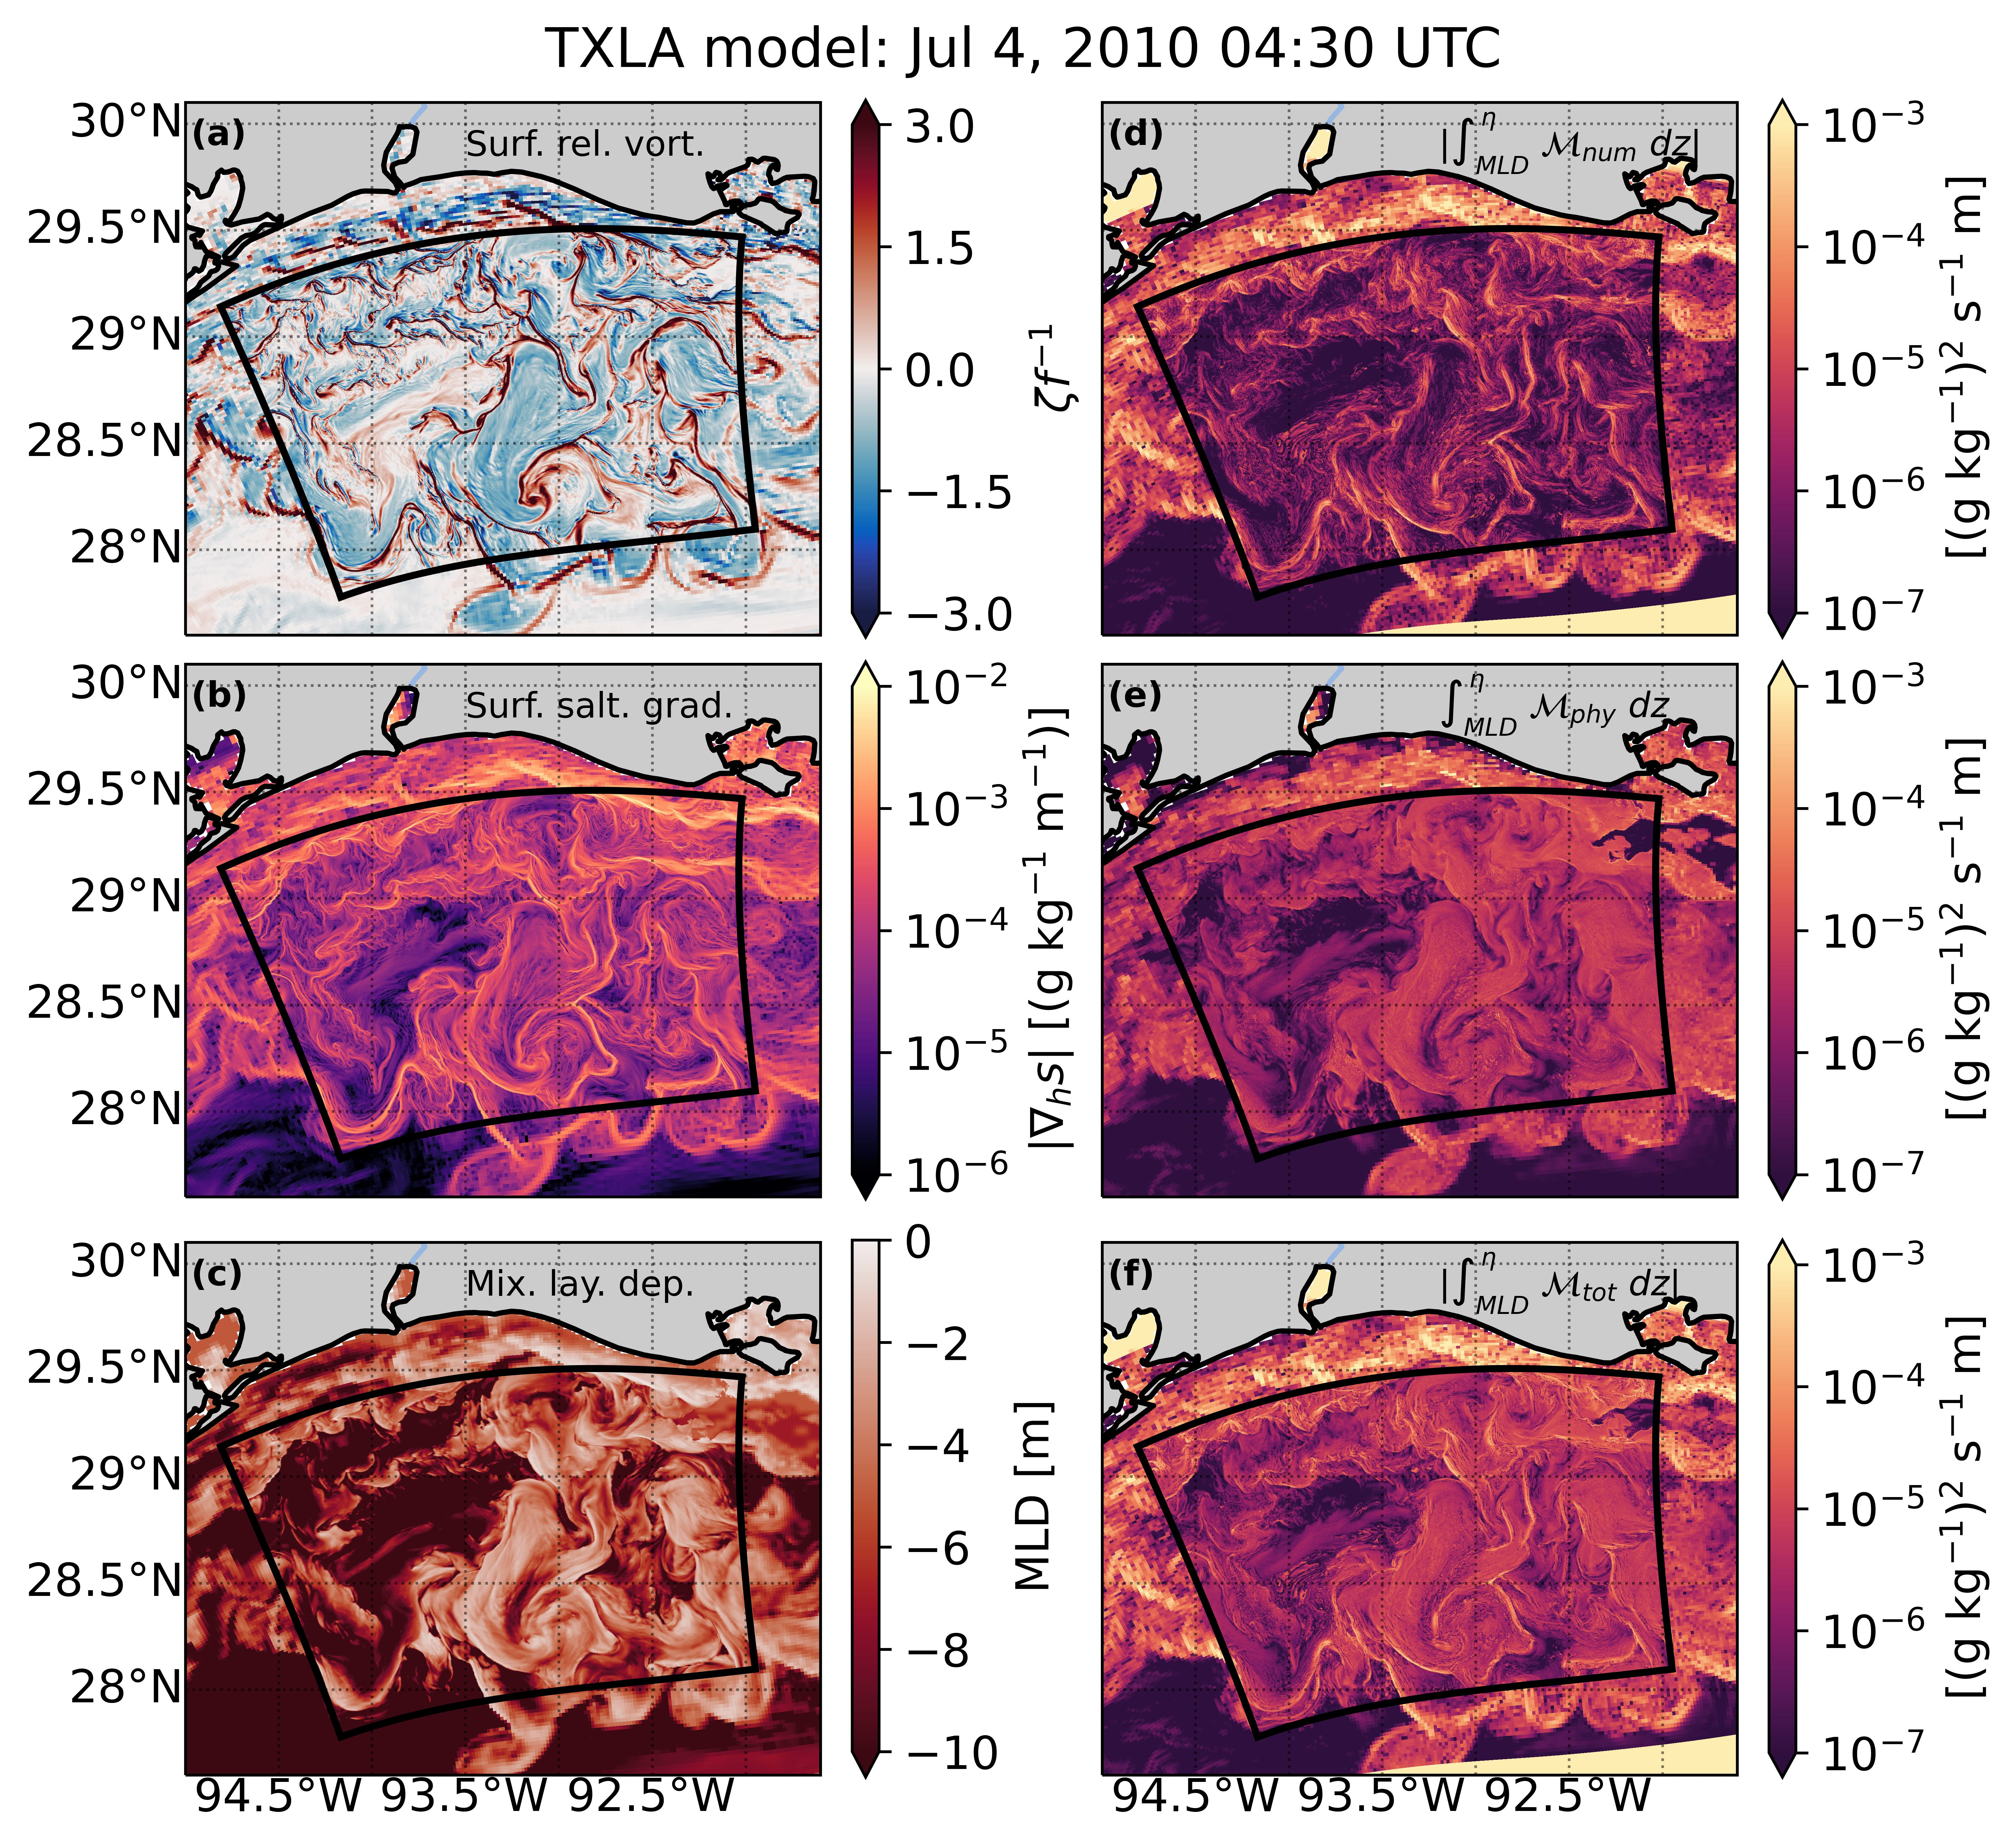
\includegraphics[width = \linewidth]{figures/shelfstrat_2024/txla_snap_int_mld.jpg}\\
    \caption{TXLA model surface $\zeta f^{-1}$ (a), $|\nabla_h s|$ (b), and mixed layer depth (MLD) (c) on July 4, 2010 04:30 UTC. The child domain is marked by the black box. $\mathcal{M}_{num}$ (d), $\mathcal{M}_{phy}$ (e), and $\mathcal{M}_{tot}$ (f) depth-integrated from the base of the mixed layer to the free surface. Note the absolute values are shown in (d) and (f) to account for negative numerical mixing. Here, bulk $\mathcal{M}_{num}/\mathcal{M}_{tot}=24$\% in the child domain. $\mathcal{M}_{num}$ is elevated near the southern boundary of the parent domain and within several bays/estuaries due to coarse grid resolution and close proximity to the open boundary. The colorbars are saturated to emphasize fronts.} \label{fig:txla_snap}
     \end{center} 
\end{figure}

The fronts, marked by normalized relative vorticity $\zeta f^{-1} > 1$, where $\zeta = \partial_x v - \partial_y u$ and $f$ is the Coriolis parameter, are characterized by sharp horizontal salinity gradients. Numerical mixing is depth-integrated from the base of the mixed layer to the free surface and compared with the physical- and total mixing. The mixed layer depth (MLD) is defined using the standard vertical density difference cutoff of 0.03 kg m$^{-3}$ \citep{de2004mixed}. As discussed previously, numerical mixing is significant at fronts due to large horizontal salinity gradients. For the child model domain in Fig. \ref{fig:txla_snap}, numerical mixing constitutes about 24\% of the total mixing. Other definitions of MLD may be used \cite[see][]{thomson2003estimating}, but these do not change the general result that the ratio of numerical- to physical mixing grows as the lower limit of integration shoals. For example, depth-integrating over the top one m of the water column to the free surface increases this ratio to 52\%. When the eddies are less perturbed by regional forcing \citep[e.g., Fig. 2 of][]{Schlichting23}, this ratio can exceed 75\%. This implies that even as the horizontal resolution is pushed towards submesoscale resolving, mixing processes in the frontal zone may be numerically driven. More broadly, this reinforces the idea that numerical mixing can dominate in regions where physical mixing is weak \citep{Kalra_2019, Wang_2021}.

The primary goal of this paper is to characterize and quantify the numerical mixing in a submesoscale eddy-resolving model, and to gain insight into how this numerical mixing impacts the larger-scale ocean state. It is difficult to address this with a realistic model due in part to the large computational cost, but also the difficulty in quantifying the difference in model states with different numerical mixing in a complex, realistic model. We therefore use an idealized model based on \citet{Hetland_2017} that captures many of the characteristics of the submesoscale eddy field seen in the realistic model. We use three different advection schemes as a way to modify the numerical mixing across different simulations. We then assess the impact of these different advection schemes through alongshore means in the idealized model -- an analysis that is not possible in the realistic model. Our primary finding is that numerical mixing suppresses the release of available potential energy, impacting the eddy field and the offshore extent of the fresh water front.


\section{Numerical models} \label{sec:model_setup}
Both models are implementations of the Regional Ocean Modeling System \citep[ROMS,][]{shchepetkin2005regional} configured as part of the Coupled-Ocean-Atmosphere-Waves-Sediment-Transport model \citep[COAWST, ver. 3.7,][]{Warner_2010}.

\subsection{Realistic ROMS model}
The two-way nested TXLA model setup is described in \citet{Schlichting23}. The sub-domain marked with a black box in Fig.~\ref{fig:txla_snap} is the higher-resolution child model (which is nested in a coarser resolution parent model): in this paper we exclusively use the child model. Only details necessary to compare with the idealized model are provided. The horizontal resolution of the child model spans from approximately 255 m close to the coast to 357 m near the offshore boundary with a mean resolution of 315 m. The model uses 30 vertical layers with functions (vtransform=2, vstretching=4) and stretching parameters ($\theta_s = 5,\theta_b=0.4$). The vertical resolution in the top m of the water column ranges from 13 cm close to the coast to 73 cm near the southern boundary, with a mean resolution of 38 cm. 
The lowest vertical resolution is about 36 m over the continental slope. As discussed above, this model exhibits significant numerical mixing near the ocean surface. To elucidate the causes and effects of this numerical mixing, we created an idealized model in a similar regime to the realistic model. 
 
\subsection{Idealized ROMS model}
The model configuration follows \citet{Hetland_2017} and is based on a water mass analysis of summer conditions over the TXLA shelf (see his Fig. 5). ROMS is configured as a reentrant shelf with periodic alongshore boundary conditions and a wall at the coast (Fig. \ref{fig:ideal_ics}). The domain is 97 km in the along- and across-shore directions with a horizontal resolution of 500 m. The vertical grid parameters are the same as the realistic model. The minimum water depth is five m at the coast and approximately 103 m at the offshore boundary with a bottom slope of 0.001. Over the initially stratified region, the vertical resolution is about 16 cm in the top one m of the water column and one m over the entire water column, with the coarsest vertical resolution being 6.8 m close to the bottom. A small amount of random noise equal to 1\% of the local depth is added to the bathymetry to force instabilities. The offshore boundary conditions for the free surface and depth-averaged currents use a Chapman-Flather combination \citep{chapman1985numerical,flather1976tidal}. The three-dimensional variables use a no gradient condition at the offshore boundary. While a no-gradient boundary condition is unrealistic, we analyze the near-inertial wind ensemble runs described in Section \ref{sec:results} before eddies interact with the offshore boundary. 

\begin{figure}[t]
    \begin{center}
    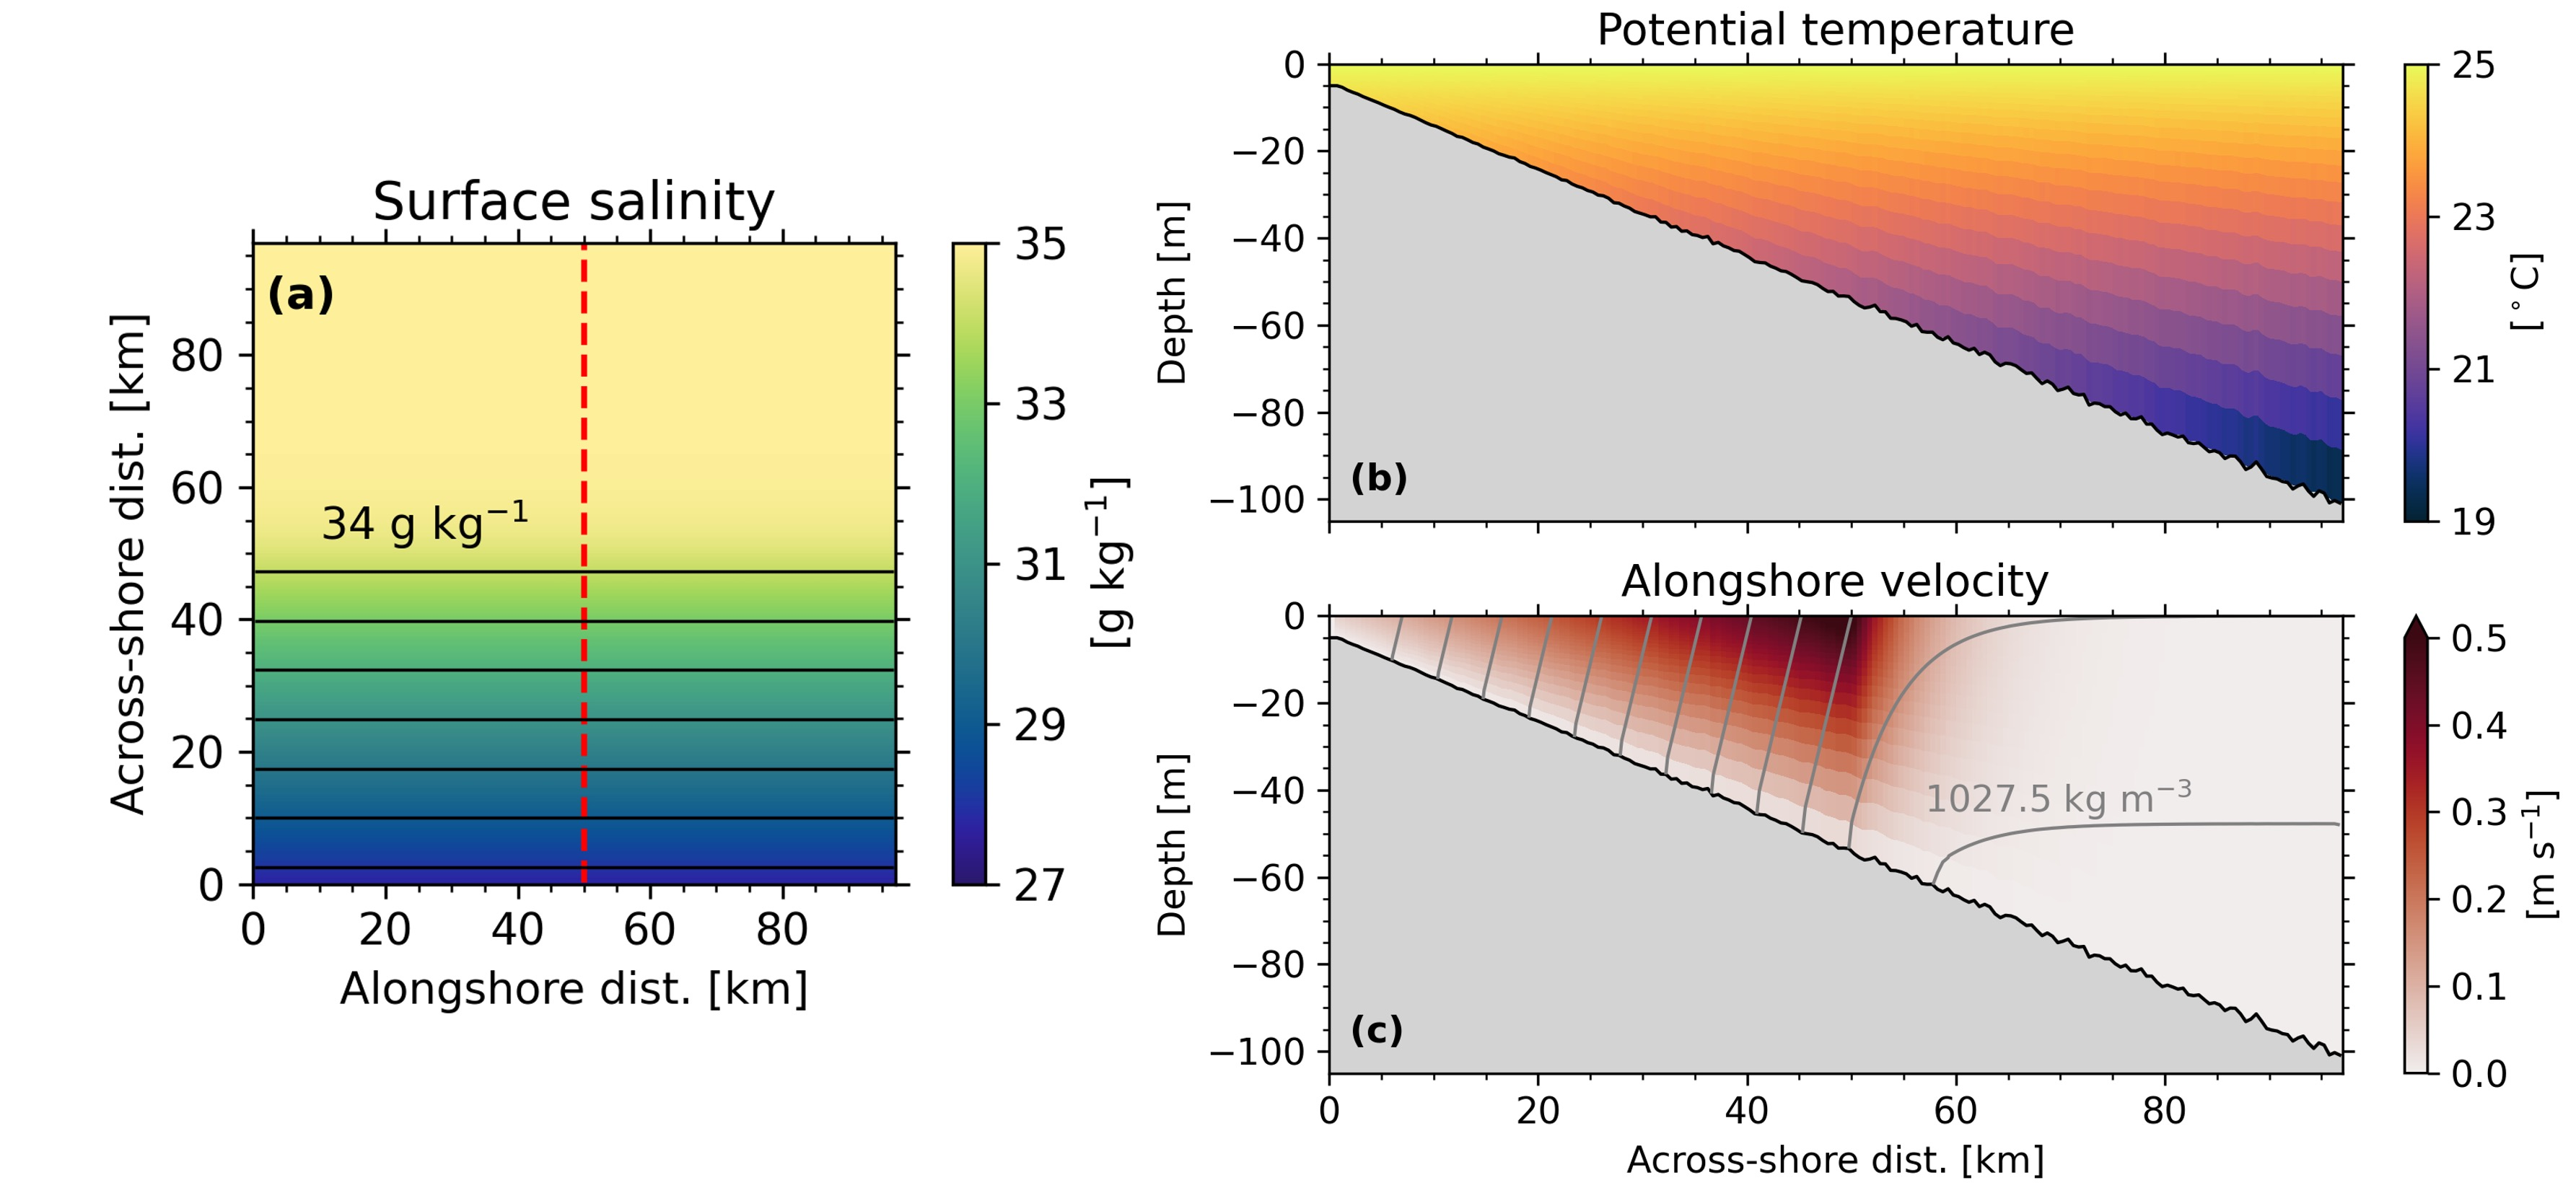
\includegraphics[width = \linewidth]{figures/shelfstrat_2024/initial_conditions_1.jpg} \\
    \caption{Idealized model initial conditions. Plan view of surface salinity (a) with isohalines overlaid every g kg$^{-1}$ and cross-sections of potential temperature (b) and alongshore velocity (c) with isopycnals overlayed every 0.5 kg m$^{-3}$. The cross-sections are shown at the red dashed line in (a).} \label{fig:ideal_ics}
     \end{center}
\end{figure}

The model is run on an $f$ plane with the Coriolis parameter $f$ set to $10^{-4}$ s$^{-1}$ ($\sim$ 43.5$^\circ$N) such that the inertial period is about 17.4 hours. Multidimensional Positive Definite Advection (MPDATA) is used for tracer advection \citep{Smolarkiewicz_1998} for all runs until specified otherwise. The $k-\epsilon$ turbulence closure scheme is used to parameterize the vertical mixing \citep{umlauf2003generic, Warner_2005}. No explicit lateral mixing scheme is prescribed. The model initial conditions (Fig. \ref{fig:ideal_ics}) are specified in terms of two non-dimensional parameters: the Richardson Number ($Ri=N^2f^2M^{-4}$) and slope Burger number $S=Nf^{-1}\alpha$. $N$ is the buoyancy frequency, $M^2$ is the magnitude of the lateral buoyancy gradients $|\left(\nabla_h b \right)^2|$, and $\alpha$ is the bottom slope. The resulting values of Ri and S are 1.0 and 0.1, respectively. The initial salinity varies only in the horizontal with a constant across-shore gradient inshore of 50 m depth with $M^2=10^{-6}$s$^{-2}$. The initial temperature field varies only in the vertical with $N^2 = 10^{-4}$s$^{-2}$. Density $\rho$ uses a linear equation of state:
\begin{equation} \label{eqn:EOS}
    \rho = 1027 \left[1+7.6 \times 10^{-4}(s-35)-1.7 \times 10^{-4} (\theta-25) \right] \, , 
\end{equation}
where $s$ is the salinity and $\theta$ is the temperature.
The alongshore flow is initialized with geostrophic vertical shear and no flow at the bottom. The bottom boundary layer uses a logarithmic velocity profile with a bottom roughness of 0.003 m.

\section{Analysis methods} \label{sec:analysis_tools}

\subsection{Energetics}
Volume-integrated energetics are used to explore how baroclinic instability affects the stratification and eddy kinetic energy. A Reynolds decomposition $\mathbf{u}=\overline{\mathbf{u}}+\mathbf{u}^\prime$ is used to divide the flow into a mean $\overline{\mathbf{u}}$ and fluctuating $\mathbf{u}^\prime$ component, with $\mathbf{u}$ denoting the horizontal velocity vector. Due to the periodic boundary condition, we follow \citet{Hetland_2017} and define $\overline{\mathbf{u}}$ with an alongshore mean:
\begin{equation}
    \overline{\mathbf{u}}=\frac{1}{L} \int_0^L \mathbf{u} \, dx
\end{equation}
such that $\mathbf{u}^\prime$ is the perturbation from the alongshore mean. The total kinetic energy ($TKE$), mean kinetic energy ($MKE$), and eddy kinetic energy ($EKE$) are defined as \citep{cushman2011introduction}:
\begin{equation} \label{eqn:tke}
    TKE = \frac{1}{2}(u^2+v^2) ,
\end{equation}
\begin{equation} \label{eqn:mke}
    MKE = \frac{1}{2}(\overline{u}^2+\overline{v}^2) ,
\end{equation}
\begin{equation} \label{eqn:eke}
    EKE = \frac{1}{2}(u^{\prime^2}+v^{\prime^2}) .
\end{equation}
Note that \citet{Hetland_2017} defined $MKE$ as a function of $\overline{u}$ only and thus $EKE$ was calculated as $\frac{1}{2}(u^{\prime^2}+v^{2})$. This is because the alongshore mean of the across-shore velocity $\overline{v}$ is initially zero and negligible without wind forcing. However, this is not the case when oscillatory alongshore wind forcing is added, so we calculate $v^\prime$ with reference to an alongshore mean. Volume-integrated versions of Eqs. \ref{eqn:tke}-\ref{eqn:eke} over the initially stratified region will be used to determine when to analyze mixing and to get an understanding of how wind forcing affects instability development. They are normalized by the initial $MKE$ ($MKE_0$) so the initial $TKE$ and $MKE$ are one. Thus, 
\begin{equation}
    TKE_n = \frac{\iiint TKE \, dV}{\iiint MKE_0 \, dV},
\end{equation}
\begin{equation}
    MKE_n = \frac{\iiint M
    KE \, dV}{\iiint MKE_0 \, dV},
\end{equation}
\begin{equation}
    EKE_n = \frac{\iiint EKE \, dV}{\iiint MKE_0 \, dV}.
\end{equation}

\subsection{Volume-averaged salinity variance}
\citet{Li_2018} showed that salinity variance can be used to characterize the stratification within a control volume. The salinity variance is also defined using a Reynolds decomposition. We split the salinity into a volume-averaged ($\overline{s}$) and fluctuating ($s_{tot}^\prime$) component such that the total variance is written as  
\begin{equation}
        s_{tot}^{\prime^2} = (s-\overline{s})^2, \, \, \xrightarrow{} \overline{s} = \frac{1}{V} \iiint s \, dV.  
\end{equation}

This can be decomposed into vertical ($s_v^{\prime^2}$) and horizontal ($s_h^{\prime^2}$) components. For example, $s_v^{\prime^2} = (s-\Tilde{s})^2$ is defined with the vertically-averaged salinity $\Tilde{s}$. After some manipulation, it follows that the volume-averaged total salinity variance can be decomposed as:
\begin{equation} \label{eqn:vavg_svar}
        \frac{1}{V} \iiint s_{tot}^{\prime^2} \, dV = \frac{1}{V} \iiint s_{h}^{\prime^2} \, dV + \frac{1}{V} \iiint s_{v}^{\prime^2} dV. 
\end{equation}
Eq. \ref{eqn:vavg_svar} is the volume-averaged version of Eq. 8 from \citet{Li_2018}. $s_h^{\prime^2}$ can be calculated by quantifying $s_{tot}^{\prime^2}$ and $s_{v}^{\prime^2}$ individually and subtracting the two. Previous studies have reported estimates of $\iiint s_{tot}^{\prime^2} \, dV$ \citep{Wang_2018, Burchard_2019}. However, this can be difficult to physically interpret because it scales with $V$. Volume-averaging alleviates this and allows for direct comparison with other estuaries and coastal regions.  

\subsection{Quantification of mixing}
Physical mixing is defined as the dissipation of salinity variance \citep{Burchard_2008, MacCready_2018}:
\begin{equation}
        \mathcal{M}_{phy} = 2 \kappa_v \left(\partial_z s \right)^2, 
\end{equation}
where $\kappa_v$ is the vertical salinity diffusivity. 

Numerical salinity mixing is calculated following \cite{Burchard_2008}:
\begin{equation} \label{eq:mnum}
        \mathcal{M}_{num} = \frac{A\{ s^2 \}-\left(A \{s \} \right)^2}{\Delta t} \quad ,
\end{equation}
where $A$ is the advection operator (i.e., MPDATA) and $\Delta t$ is the online timestep. While \citet{Klingbeil_2014} improves the \citet{Burchard_2008} algorithm, it is not coded into the ROMS source code. $\mathcal{M}_{num}$ and $\mathcal{M}_{phy}$ are calculated online so errors associated with offline analysis do not contaminate the calculations \citep{Schlichting23}.

\subsection{2D Frontogenesis function}
Future studies may benefit from understanding how $\mathcal{M}_{num}$ changes as horizontal tracer gradients are sharpened by frontogenesis and weakened by frontoloysis. One way to conceptualize this is with the frontogenesis function $FGF$ \citep{hoskins1982mathematical, mcwilliams2021oceanic}. In two-dimensions, this describes whether advective processes are sharpening ($FGF>0$) or weakening ($FGF<0$) horizontal buoyancy gradients. $FGF$ is defined as the dot product of the tracer gradients with their Lagrangian rate of change. While typically expressed in terms of lateral buoyancy gradients, we write $FGF$ in terms of salinity because surface stratification is provided only by salinity:
\begin{equation} \label{eqn:fgf_2d}
        FGF = \frac{1}{2}\frac{D}{Dt} \left(\nabla_h s \right)^2,
\end{equation}
where $\frac{D}{Dt} = \partial_t(.) + \mathbf{u}_h \cdot \nabla_h (.)$ is the material derivative excluding the vertical term. 

Eq. \ref{eqn:fgf_2d} can be normalized so that it may compared directly with other dynamical properties. For example, \citet{barkan2019role} showed that divergence $\delta  = (\partial_x u + \partial_y v)$ is a dominant parameter driving submesoscale frontogenesis. $FGF$ can be normalized by $f$ such that it may be compared to a rotational timescale. $FGF$ can be further normalized by $\nabla_h s$, which we define as the normalized frontogenesis function $nFGF$:
\begin{equation} \label{eqn:fgf_norm}
    nFGF = \frac{1}{2f \left(\nabla_h s \right)^2}\frac{D}{Dt} \left(\nabla_h s \right)^2,
\end{equation}
which is $\mathcal{O}(1)$ when submesoscale frontogenesis and frontolysis occurs. Thus, Eq. \ref{eqn:fgf_norm} describes the time rate of change of the distance between two isohalines relative to the Coriolis parameter. In other words, the normalized rate of cross-frontal convergence and divergence. For example, $nFGF=1$ indicates horizontal salinity gradients will collapse over one rotational timescale. $nFGF = -1$ indicates a front will expand over a rotational timescale. 

\section{Results} \label{sec:results}
\subsection{Unforced- and base case}
We start with a brief description of the near-inertial wind ensemble then compare the temporal evolution of the instabilities between the unforced- and base case. An overview of how wind forcing affects properties related to mixing in other ensemble members are provided in the appendix because they are not directly related to the primary objective of this study. A total of 15 ensemble members, each with different wind forcing, were run for 20 days (Fig. \ref{fig:wind_ensembles}). Each member is named according to the amplitude of the near-inertial (0.92$f$) alongshore wind stress $\tau_0^x$. The spatially-uniform wind stress $\tau^x$ is calculated as
\begin{equation}
    \tau^x = \tau_0^x \sin(0.92 f t) \, , 
\end{equation}
where $t$ is time. The first three days are set to zero so wind forcing starts as the instabilities begin forming (Fig. \ref{fig:time_series_base}). The wind stress is prescribed to mimic the near-resonance between the diurnal winds over the TXLA shelf and the regional inertial frequency \citep{Qu_2022_NIW}. The same bathymetry is used in all ensemble members.

\begin{figure}[t!]
    \begin{center}
    \includegraphics[width = 0.9\linewidth]{figures/shelfstrat_2024/time_series_shelf_overview_vavg.jpg}\\
    \caption{Comparison between the base- and unforced case. (a) Alongshore wind stress $\tau_x$ prescribed at each surface grid cell. (b) Normalized, volume-integrated energetics as defined in text. (c) Volume-averaged $\mathcal{M}_{num}$ and $\mathcal{M}_{phy}$. The absolute value is taken to account for negative volume-integrated $\mathcal{M}_{num}$ before the instabilities form. As in (c), but depth-integrated from the base of the mixed layer to the free surface (d) and from the top one m to the free surface (e). (f) Volume-averaged salinity variance decomposition as defined in Eq. \ref{eqn:vavg_svar}. The shaded areas indicate time used for computation of bulk values.}\label{fig:time_series_base}
     \end{center}
\end{figure} 

The base case (0.1 Pa ensemble member, Fig. \ref{fig:time_series_base}) was identified as the ensemble member with the maximum ratio of volume-integrated $\mathcal{M}_{num}$ to $\mathcal{M}_{phy}$ (Fig. \ref{fig:wind_ensembles} d). The base case features a $\tau_x$ amplitude that is slightly more energetic than the magnitude of the diurnal wind stress amplitude in the realistic simulation. However, as we show later (Fig. \ref{fig:jpdf}), the representation of frontogenesis and frontolysis is statistically similar to the realistic model. By selecting the ensemble member with maximum $\mathcal{M}_{num}$ to $\mathcal{M}_{phy}$, we assume it is easier to identify the larger-scale impacts of $\mathcal{M}_{num}$ on the solution with the tracer advection experiments. All quantities hereafter are analyzed inshore of the initially stratified region, indicated by the black contours in Fig. \ref{fig:ideal_ics} (a). 

Normalized volume-integrated energetics for the case with no wind forcing are shown by dashed-dotted lines in Fig. \ref{fig:time_series_base} (b). As indicated by $EKE_n$ and consistent with \citet{Hetland_2017}, the eddy field in the unforced case forms as an organized disturbance after day three. By day ten, the instabilities are mature and never interact with offshore boundary. The $TKE$ and $MKE$ decrease as the instabilities develop due to the bottom friction, which provides a forward cascade of energy via dissipation in the bottom boundary layer. 

Volume-averaged $\mathcal{M}_{phy}$ and $\mathcal{M}_{num}$ are shown for three depth ranges: 1) The entire water column (Fig. \ref{fig:time_series_base} c), 2) from the base of the mixed layer to the free surface (Fig. \ref{fig:time_series_base} d), and the top one m to the free surface (Fig. \ref{fig:time_series_base} e). All quantities are volume-averaged so changes to $V$ for the different depth ranges are taken into account. For all depth ranges, both mixing quantities increase as the instabilities form, but exhibit different temporal variability. However, bulk values are computed with volume-integrals because we are interested in the integrated effects that changing the wind forcing has on mixing. From days 7.5-15, the ratio of bulk $\mathcal{M}_{num}$ to $\mathcal{M}_{phy}$ is 6.5\%. For the entire water column, $\mathcal{M}_{phy}$ increases until the instabilities are mature then reaches near steady-state as they penetrate further into the water column and relax the mean flow. $\mathcal{M}_{num}$ maximizes near day seven then decreases for the remainder of the simulation as $|\nabla_h s|$ weakens.

Volume-averaging from the base of the mixed layer increases the ratio of bulk $\mathcal{M}_{num}$ to $\mathcal{M}_{phy}$ to 24.9\%, indicating that numerical mixing becomes more important in the mixed layer. From days 8-11, $\mathcal{M}_{num}$ declines by over an order of magnitude before returning to previous levels. This variability is not seen in time series of $\mathcal{M}_{num}$ for the ensemble members with wind forcing, which all reach a near periodic state in days 8-11. Identifying the exact cause of this decrease is beyond the scope of this paper. $\mathcal{M}_{phy}$ reaches steady state on day ten as with the entire water column. Over the top one m of the water column, $\mathcal{M}_{num}$ rapidly increases as the eddies develop and is comparable to $\mathcal{M}_{phy}$ for froms Days 7.5-15, then gradually declines as the fronts are dissipated by bottom friction. The ratio of bulk $\mathcal{M}_{num}$ to $\mathcal{M}_{phy}$ increases to 104.8\%. These results validate the arguments suggested in Section \ref{sec:intro}; that is, even in a 500 m resolution idealized model, mixing processes near the frontal zone may be driven by $\mathcal{M}_{num}$. 

Energetics and mixing rates are related to the volume-averaged salinity variance. Until day four, $s_{tot}^{\prime^2}$ consists only of $s_{h}^{\prime^2}$ due to the initial conditions, as shown in Fig. \ref{fig:time_series_base} (f).  $s_{tot}^{\prime^2}$ slightly increases until the instabilities mature on day ten as the isopycnal slope is reduced.  $s_{h}^{\prime^2}$ is gradually converted to $s_{v}^{\prime^2}$ via differential advection of horizontal salinity gradients \citep{Li_2018} and restratification by mixed layer instabilities \citep{boccaletti2007mixed}. As the eddies are dissipated by bottom friction, the water column is mixed horizontally such that $s_{h}^{\prime^2}$ decreases. In the estuarine community, this process is referred to as tidal straining \citep{simpson1990tidal}. The key difference in our model is this process is forced by submesoscale baroclinic instabilities -- not tidal forcing. $s_{tot}^{\prime^2}$ is $\mathcal{O}(3 \text{(g kg}{^{-1}})^{2})$, less than half that of the TXLA child model domain (Fig. 7 of \citet{Schlichting23}) and about an order of magnitude less than partially mixed estuaries such as the Hudson or Changjiang \citep{Li_2018, Warner_2020}. This is due to the small salinity range used to specify the initial conditions $s = [\sim 28,35]$, whereas over the TXLA shelf $s = [0,\sim 37]$. 

The solid lines in Fig. \ref{fig:time_series_base} represent the same quantities discussed above for the base case, which has a wind stress amplitude of 0.1 Pa. The winds energize the velocity field, as shown by the normalized energetics (Fig. \ref{fig:time_series_base} b). Winds also increase $\mathcal{M}_{phy}$ and $\mathcal{M}_{num}$ for all vertical limits of integration. The exception is $\mathcal{M}_{phy}$ vertically integrated over the top one m because the mean vertical salinity gradient is decreased by the winds (e.g., Fig.  \ref{fig:wind_ensembles}). The nonlinear superinertial oscillations shown in the volume-averaged mixing quantities are qualitatively related to deepening of the mixed layer (not shown) and not discussed further. The ratio of bulk $\mathcal{M}_{num}$ to $\mathcal{M}_{phy}$ over the whole water column, base of the mixed layer, and top one m are as follows: 15.4\%, 49.3\%, and 210.8\%. 

Additionally, $s_{tot}^{\prime^2}$ and $s_{v}^{\prime^2}$ are lower than the unforced case because $\mathcal{M}_{phy}$ destroys vertical salinity variance by definition. However, $s_{h}^{\prime^2}$ remains comparable to the unforced case. The wind-forced eddies extend further beyond the initially stratified region and features sharper fronts relative to the unforced case (as approximated by $|\nabla_h s|$, Fig. \ref{fig:wind_ensembles} b).

To qualitatively demonstrate the base case eddies are comparable with the realistic model, Fig. \ref{fig:base_case_plan} shows plan view plots of $\zeta f^{-1}$, $|\nabla_h s|$, $\delta f^{-1}$, and $nFGF$ on day 15 at the surface. Snapshots of $\zeta f^{-1}$ in the realistic model when eddies are well developed are found readily in previous studies \citep{Hetland_2017, Kobashi_2020, Qu_2022_NIW}. As with the realistic model, $|\mathcal{M}_{num}|$ is strongest at fronts by several orders of magnitude and is associated with sharp $|\nabla_h s|$. As \citet{barkan2019role} suggests, $nFGF$ is negatively correlated with $\delta f^{-1}$. That is, frontogenesis is associated with convergent flows and frontolysis is associated with divergent flows.

\begin{figure}[t!]
    \begin{center}
    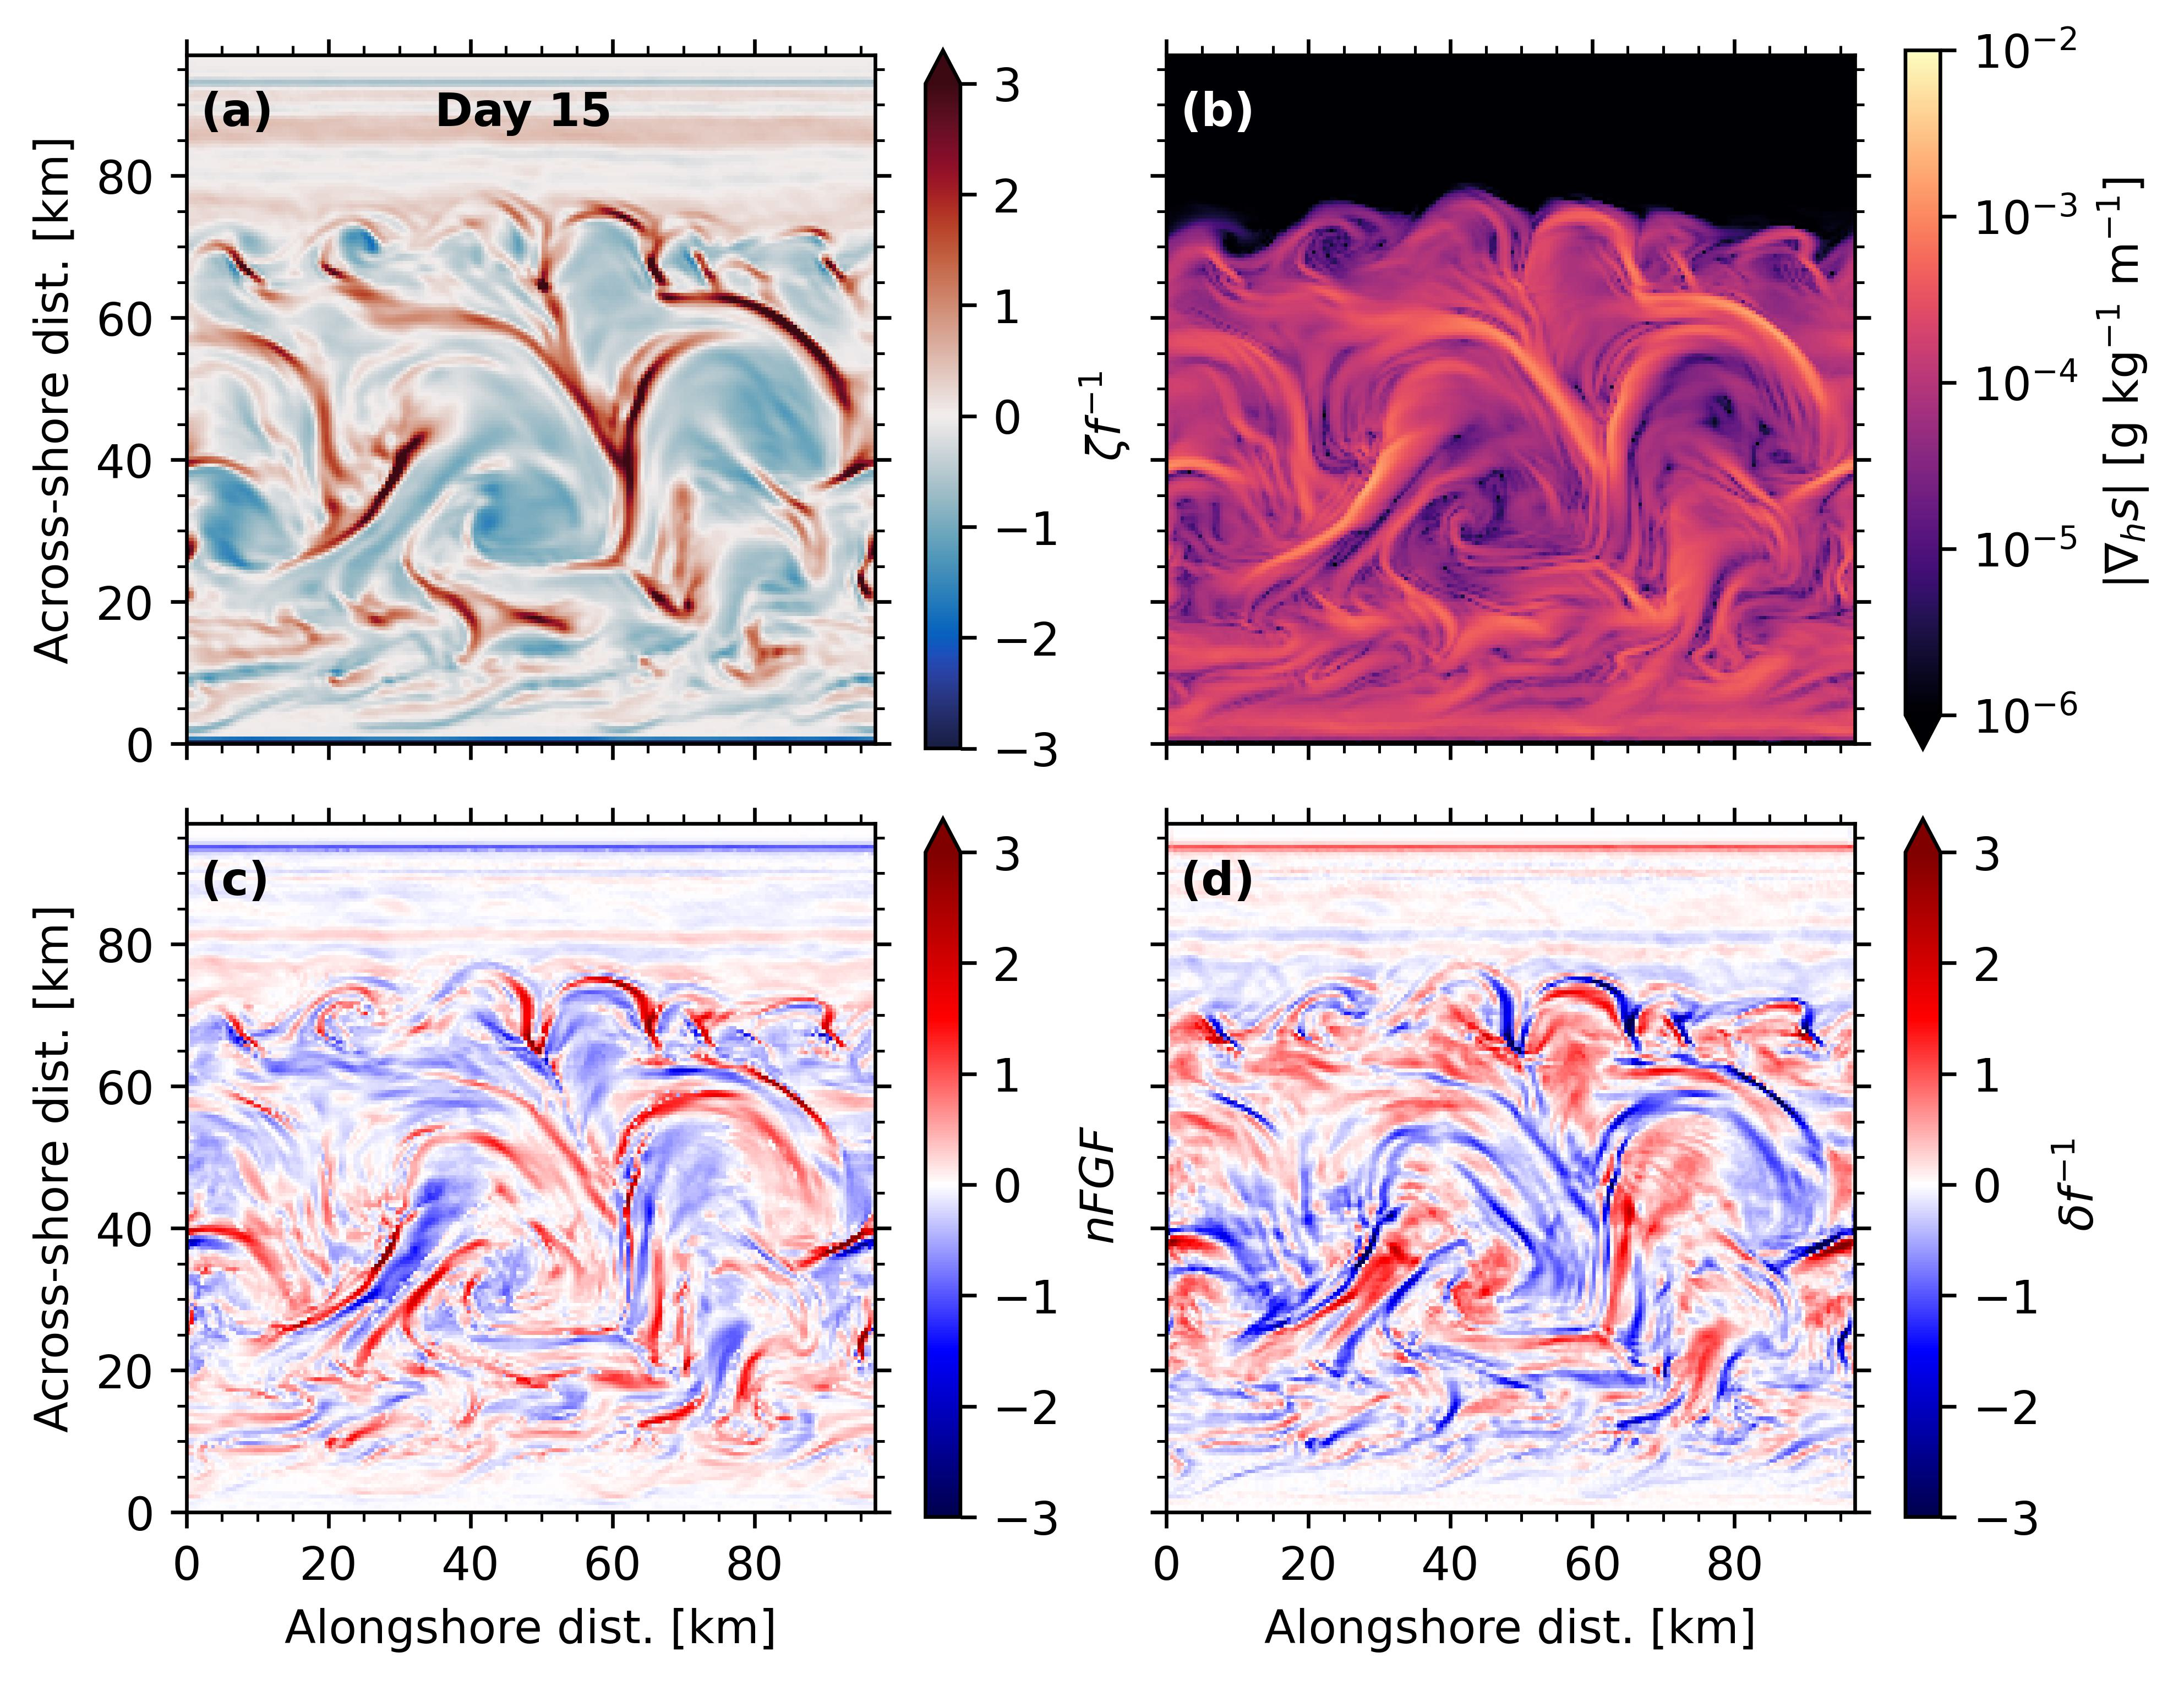
\includegraphics[width = \linewidth]{figures/shelfstrat_2024/surface_properties_day15.jpg}\\
    \caption{Plan view plots of surface $\zeta f^{-1}$ (a), $|\nabla_h s|$ (b), $nFGF$ (c), and $\delta f^{-1}$ (d) for the base case on day 15 as defined in text. $|\nabla_h s|$ values in (b) offshore of the instabilities are set to $10^{-6}$ g kg$^{-1}$ m$^{-1}$ to saturate the colorbar because they are poorly defined.}
    \label{fig:base_case_plan}
     \end{center}
\end{figure}

A statistical comparison between the realistic model and base case is shown with joint probability density functions (JPDFs) of $\mathcal{M}_{num}$ and $nFGF$ in the surface layer in Fig. \ref{fig:jpdf}. The absolute value of $\mathcal{M}_{num}$ is taken to account for negative values. The cyan line marks the maximum probability of $\mathcal{M}_{num}$ in each $nFGF$ bin sorted by active fronts ($\zeta f^{-1}>1$). The yellow line displays all cells in the surface layer. The TXLA model JPDF was constructed using a week of model output where the eddies are relatively unperturbed by various forcing (compare Fig. \ref{fig:txla_snap} to Fig. 2 of \citet{Schlichting23}). 

\begin{figure}[t!]
    \begin{center}
    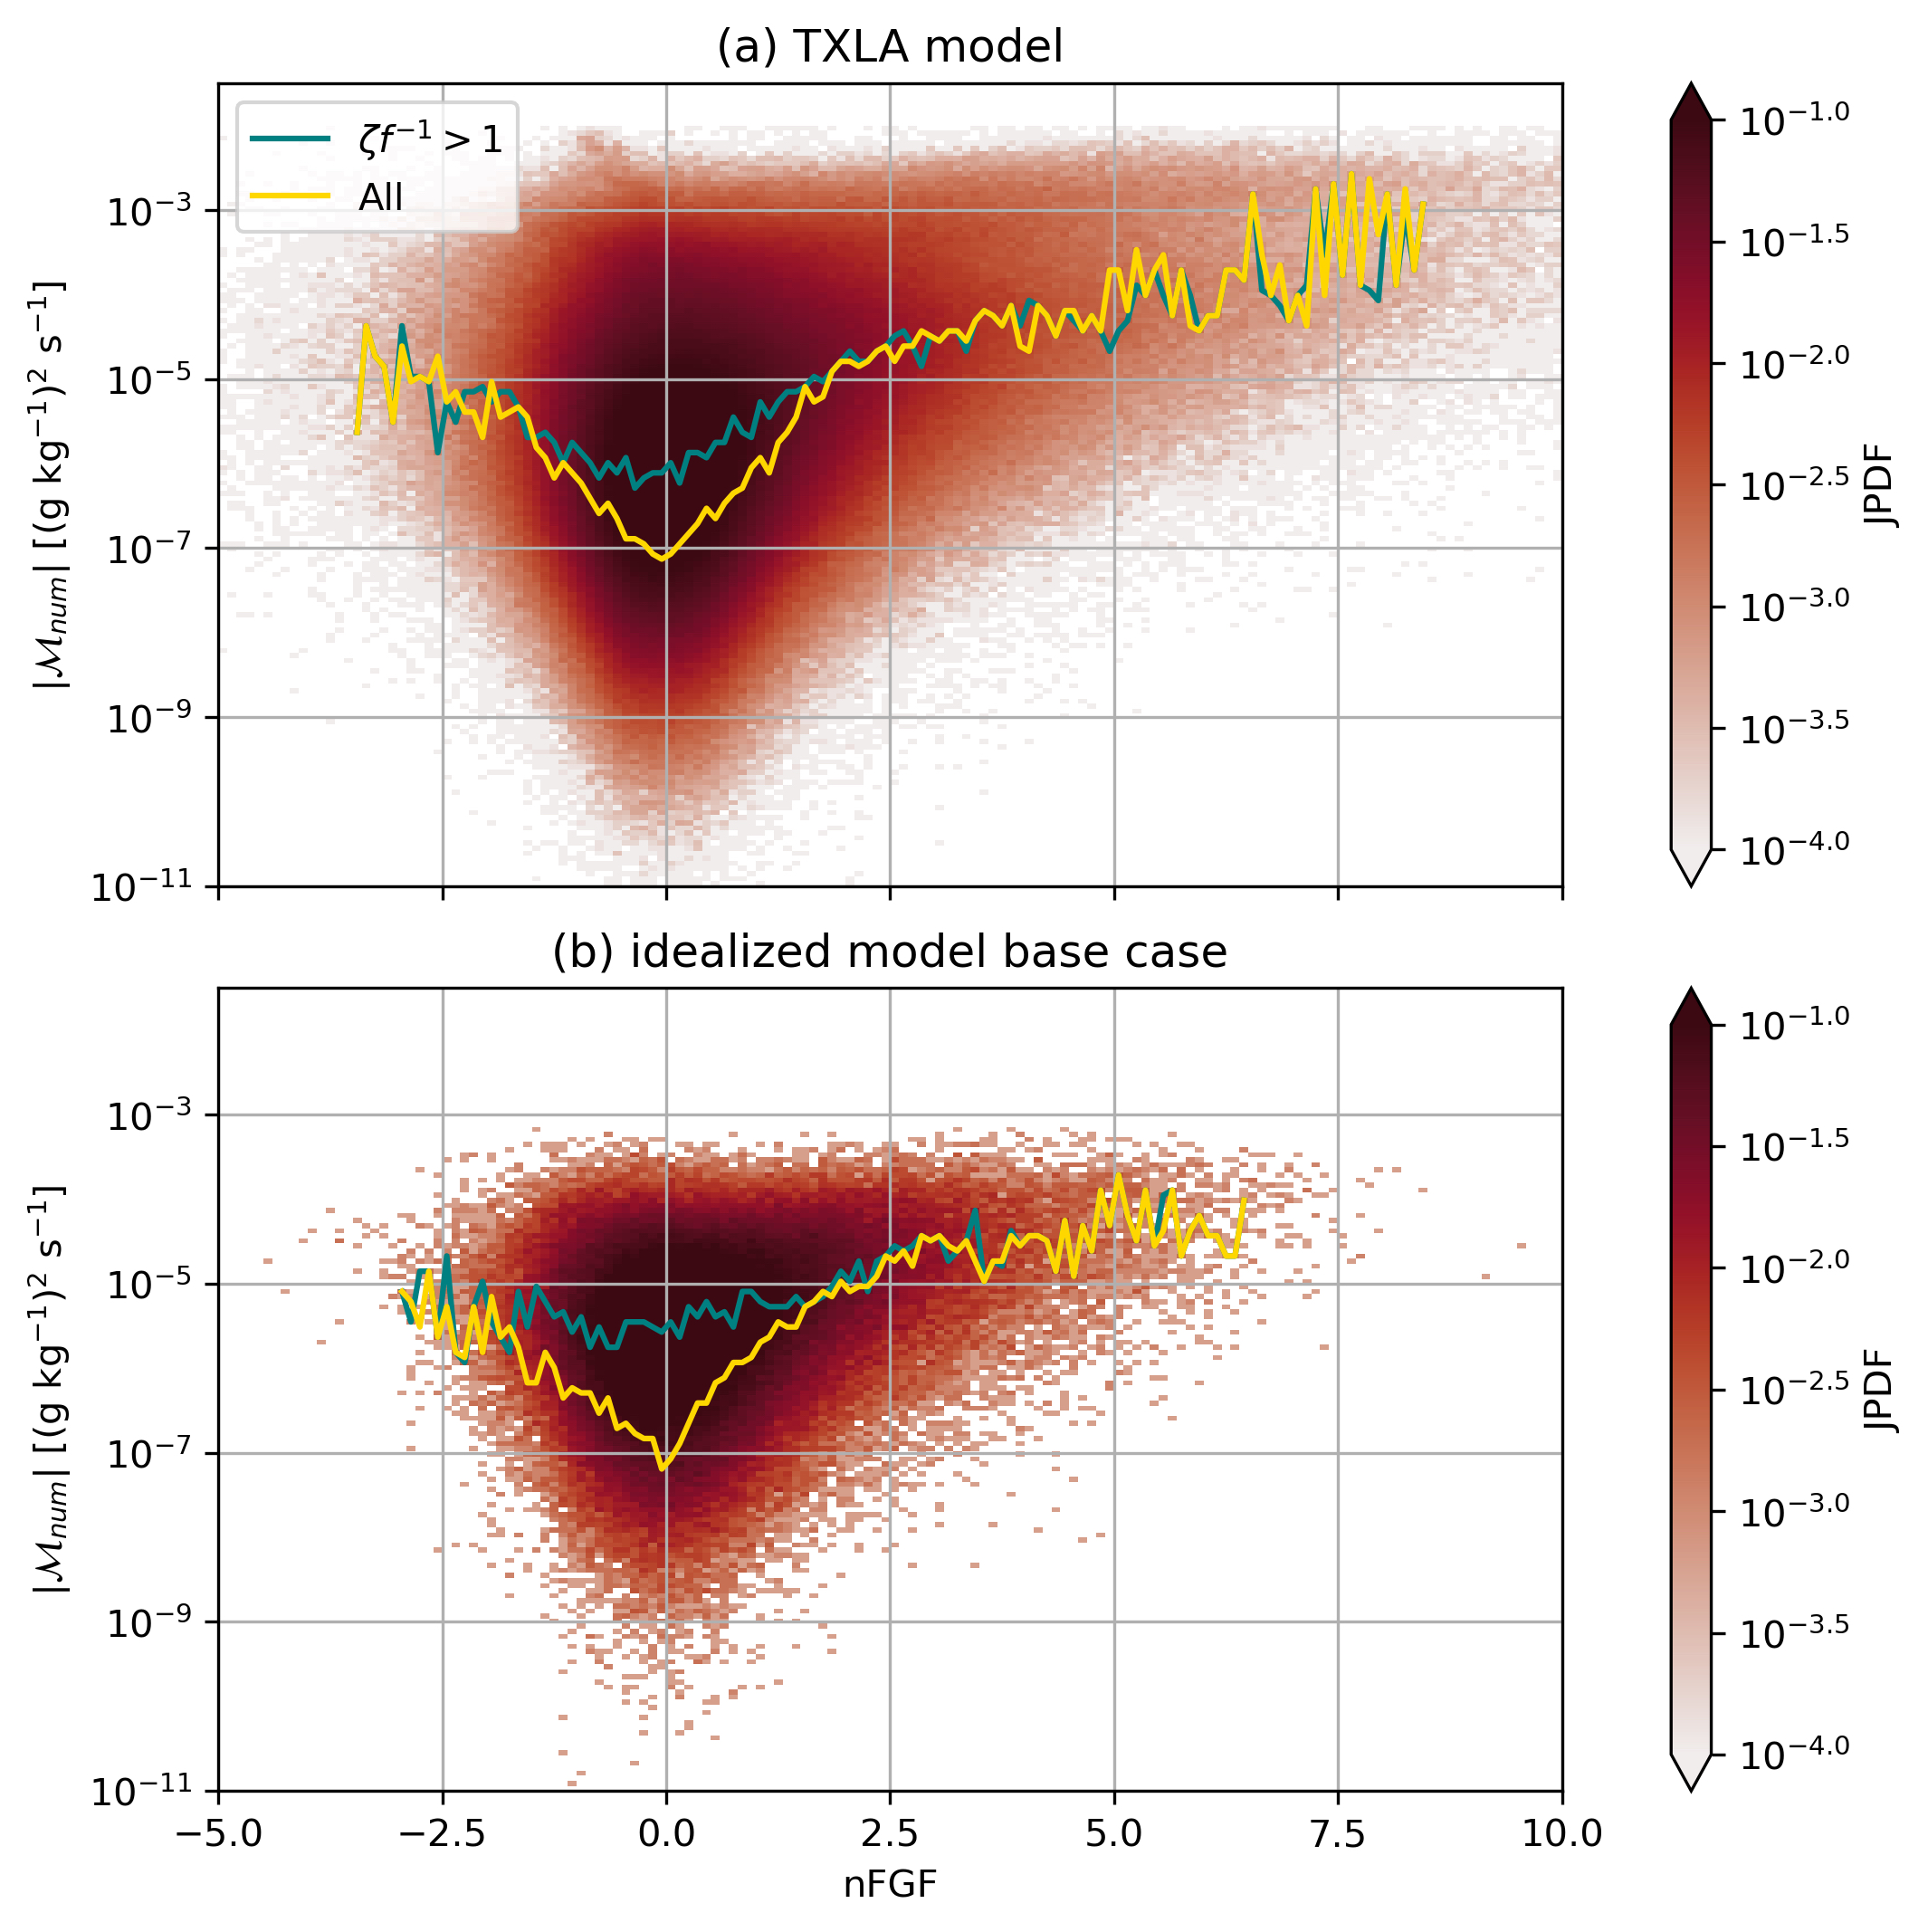
\includegraphics[width = 0.9\linewidth]{figures/shelfstrat_2024/txla_shelfstrat_jpdf.jpg}\\
    \caption{Joint probability density function (JPDF) of surface $|\mathcal{M}_{num}|$ and $nFGF$  for the realistic model from June 20-26, 2010 (a). The cyan line highlights the maximum value of the JPDF in each $nFGF$ bin sorted by active fronts ($\zeta/f>1$)  and the yellow line marks the same calculation but the entire surface layer. (b) Same as (a), but for the base case from days 7.5-15 inshore of the initially stratified region.  In (b), we removed the first three across-shore boundary points near the coastal wall due to strong convergence and divergence regions generated by the winds.}\label{fig:jpdf}
     \end{center}
\end{figure}

Several conclusions are drawn from Fig. \ref{fig:jpdf}: 1) the strongest occurrences of frontogenesis produce the sharpest horizontal salinity gradients and thus the strongest $\mathcal{M}_{num}$, 2) numerical mixing experiences the largest variability when frontogenesis and frontolysis are weak (i.e., $nFGF \sim [-1,1]$), which constitutes the majority of grid cells in the surface layer, 3) frontogenesis and frontolysis in the base case is representative of the realistic model, and 4) $nFGF$ is skewed towards frontogenesis. An interesting result is that $\mathcal{M}_{num}$ is significant even for strongly frontolytic processes. This reinforces the idea that lateral tracer gradients are a dominant parameter modulating $\mathcal{M}_{num}$, even if those gradients are being instantaneously weakened. In addition, the base case features smaller $\mathcal{M}_{num}$ and $nFGF$ ranges due to coarser lateral resolution and a smaller salinity range (see Section \ref{sec:model_setup}). The impacts of lateral resolution on $\mathcal{M}_{num}$ are further elucidated by cyan lines, where weak frontogenesis and frontolysis feature $\mathcal{M}_{num}$ maximum in each $nFGF$ bin (Fig. \ref{fig:jpdf} b) about half an order of magnitude stronger than the same range for the realistic model (Fig. \ref{fig:jpdf} a). In addition, the maximum $\mathcal{M}_{num}$ in each $nFGF$ bin for the entire surface layer converges to same quantity sorted by fronts when $|nFGF| \sim 2$. While determining a proper scaling between $\zeta f^{-1}$ and $nFGF$ or $\delta f^{-1}$ is beyond the scope of this paper, it makes intuitive sense for strong fronts and eddies to be present in regions of strong frontogenesis and frontolysis. 

\subsection{Tracer advection experiments} \label{sec:tadv_exp}
Next, we study the sensitivity of the base case with three tracer advection schemes available in the COAWST source code. The schemes used are MPDATA \citep{smolarkiewicz1984fully, Smolarkiewicz_1998}, third-order upwind in the horizontal with a vertical fourth-order centered scheme \citep[U3HC4,][]{shchepetkin1998quasi}, and third high-order spatial interpolation at the middle temporal level with a total variation diminishing scheme \cite[HSIMT,][]{wu2010advection, wu2023evaluation}. MPDATA is second order accurate but features anti-diffusive properties. \citep{Kalra_2019} also studied the sensitivity of $\mathcal{M}_{num}$ and $\mathcal{M}_{phy}$ in four idealized test cases using COAWST with the same schemes. An overview of the schemes can be found in their Section 2.2 and references therein.

We conduct 30 day ensemble runs of the base case by varying the model bathymetry to ensure differences between advection schemes are robust. That is, 1\% random noise added to the bathymetry is regenerated for each ensemble member. 95\% confidence intervals of volume-integrated, ensemble-averaged energetics and mixing quantities are provided to characterize the variability (denoted with an overbar). All quantities in Fig. \ref{fig:tadv_vol_int} are smoothed with a 16 hour rolling mean (denoted with angle brackets) to remove the primary oscillations caused by the wind and improve readability. We used a larger across-shore domain (194 km) so the eddies never interact with boundary. Volume integration was performed from the coast to 97 km across-shore, which represents the boundary of the original domain. In addition, the eddies from several ensemble members approximately reach this location by Day 30 (Fig. \ref{fig:isohalines}). We deemed eight ensemble members sufficient to capture variability caused by changing the bathymetry noise, as shown by the confidence intervals of each quantity shown in Fig. \ref{fig:tadv_vol_int}. 

\begin{figure}[t!]
    \begin{center} 
    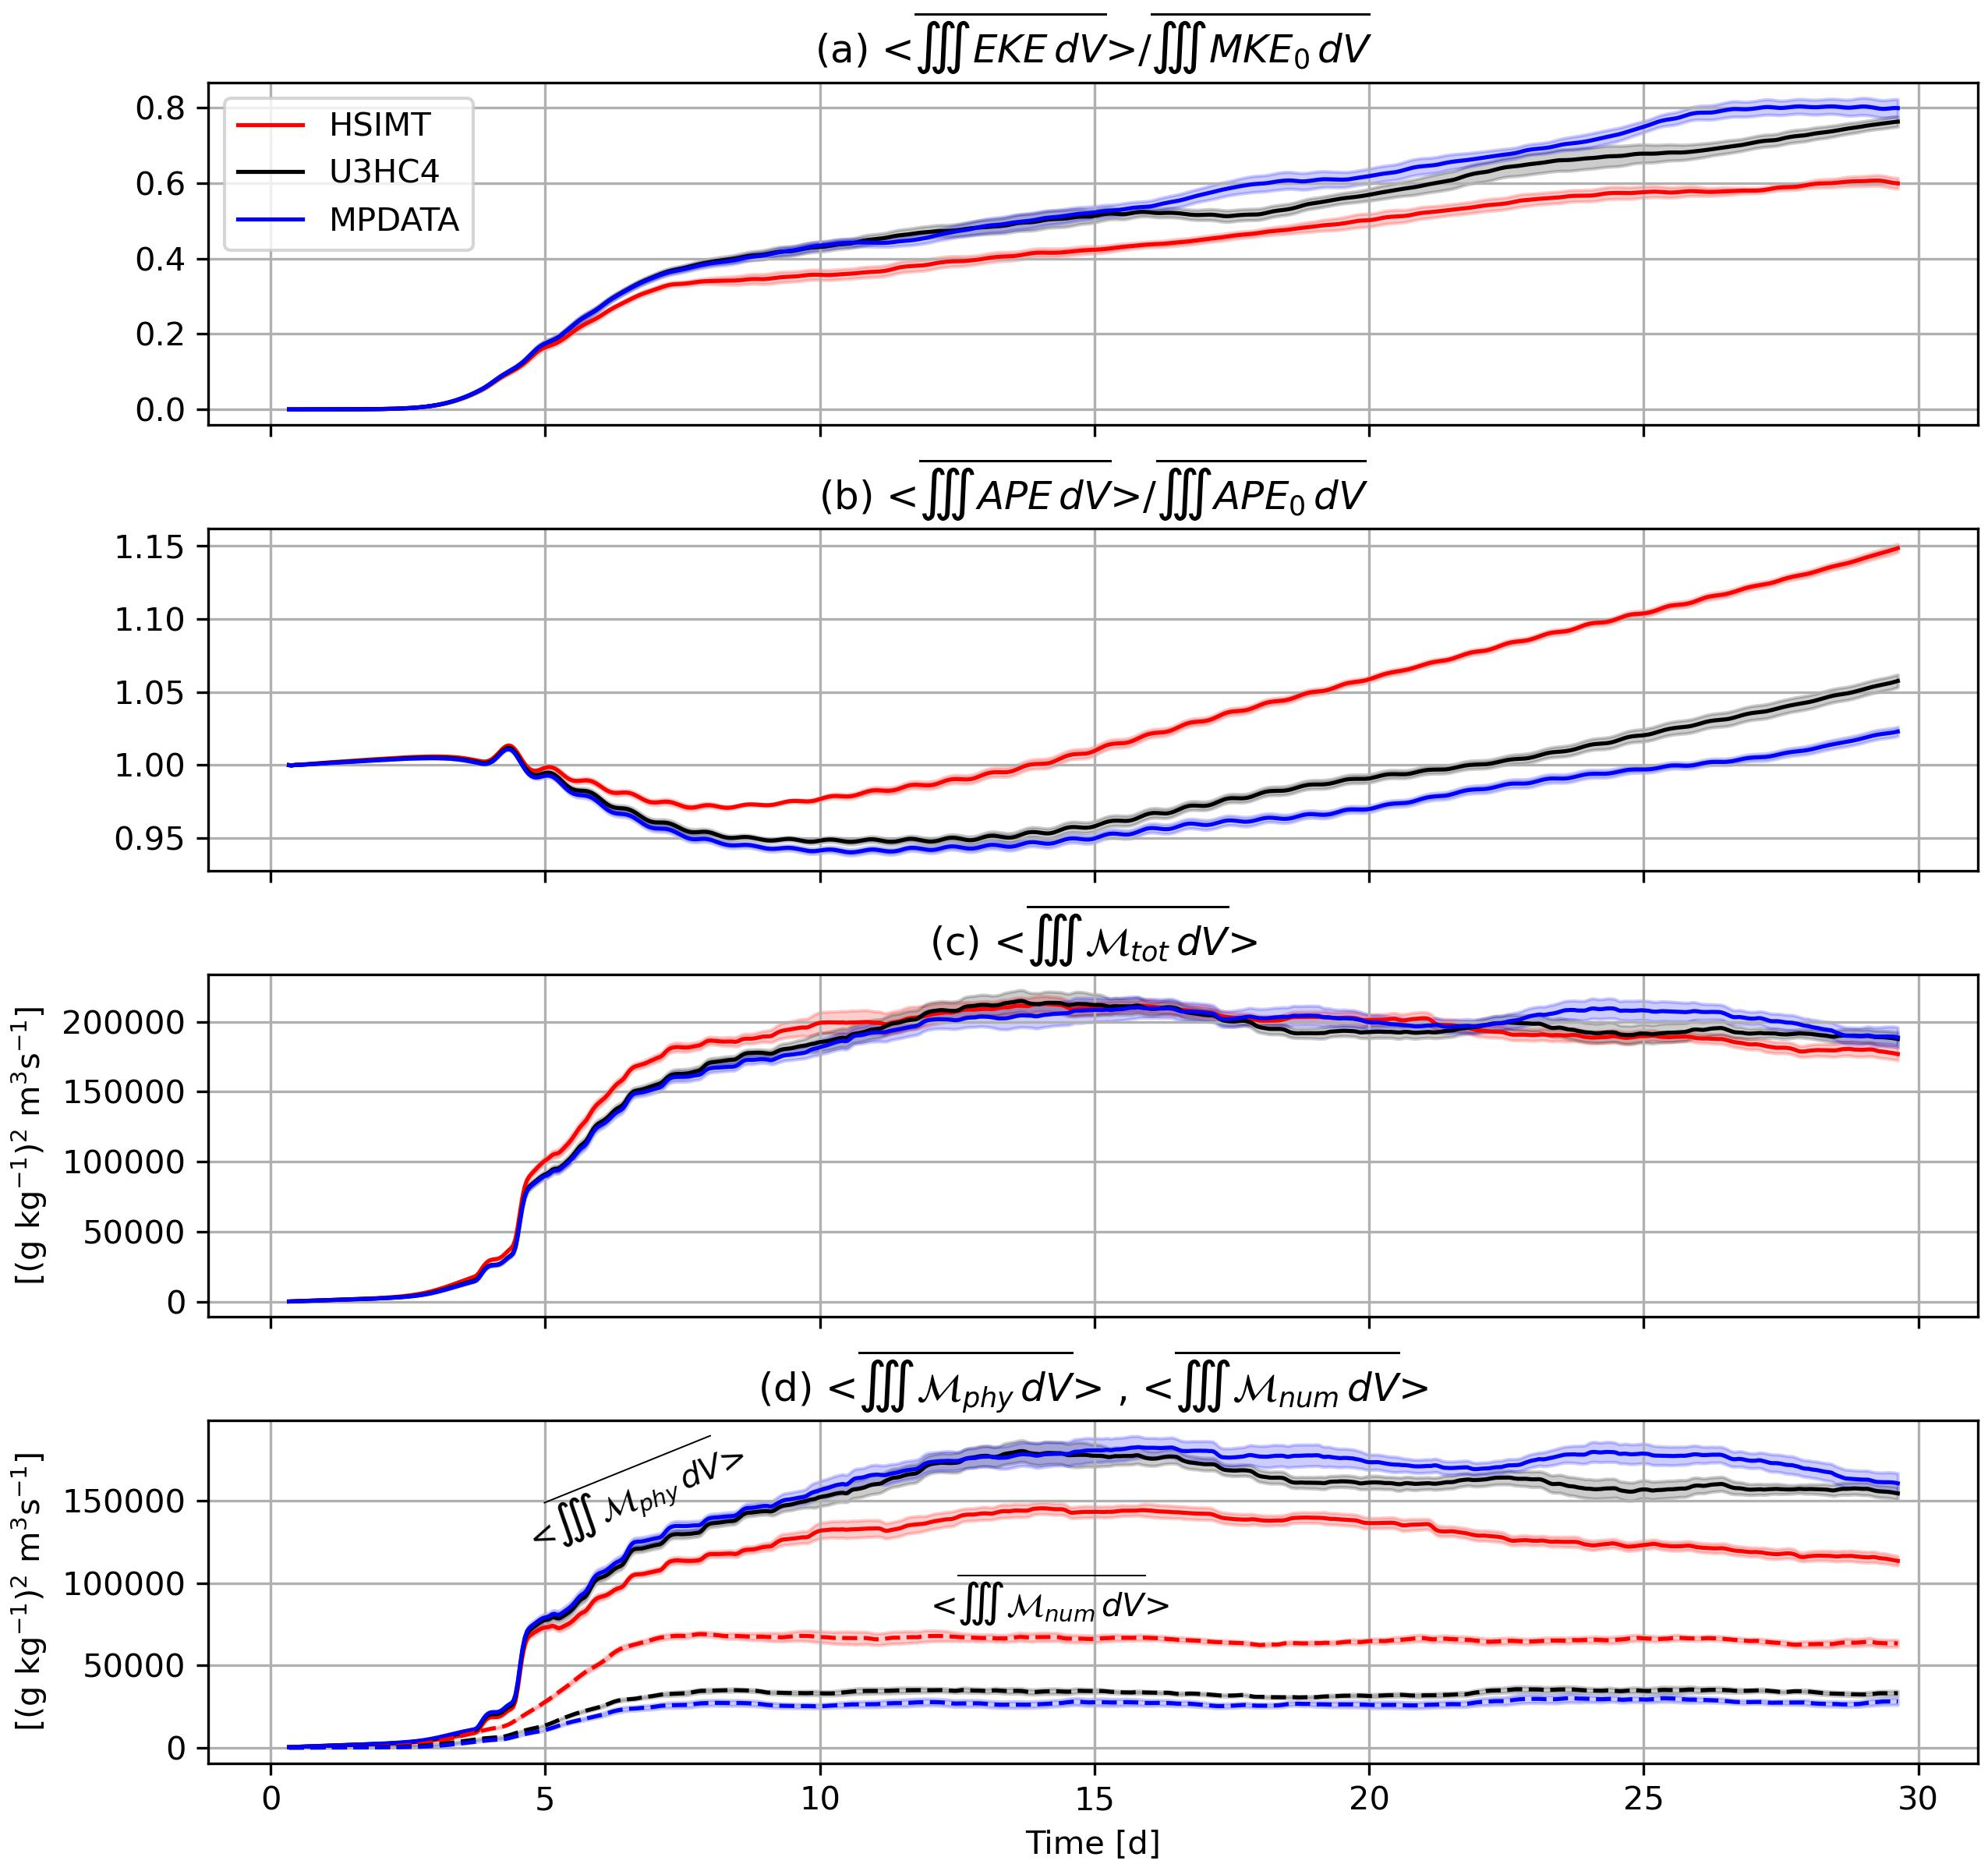
\includegraphics[width = 0.9\linewidth]{figures/shelfstrat_2024/tadvection_vol_int_ens.jpg}\\
    \caption{Time series of $EKE_{n,ens}$ (a), $APE_{n,ens}$ (b), $\mathcal{M}_{tot, ens}$ (c), and $\mathcal{M}_{phy,ens}$ and $\mathcal{M}_{num,ens}$ (d) as defined in text. The angle brackets denote a 16 hour rolling mean and the overline denotes an ensemble average. The shaded areas represent values within the 95\% confidence intervals about the ensemble means. In (d), $\mathcal{M}_{phy,ens}$ is shown with solid lines and $\mathcal{M}_{num,ens}$ is shown with dashed lines.} \label{fig:tadv_vol_int}
     \end{center} 
\end{figure}

We start with analysis of the double-averaged, volume-integrated $EKE$: 
\begin{equation}
    EKE_{n,ens} = \langle \overline{\iiint EKE \, dV }\rangle \left[\overline{\iiint MKE_0 \, dV}\right]^{-1}.
\end{equation}

Differences between schemes are detectable shortly after the eddies begin forming. HSIMT features the lowest $EKE_{n,ens}$ throughout the simulation. By Day 30, HSIMT's ensemble-averaged $EKE_{n,ens}$ is nearly 25\% less than the other schemes. The confidence intervals of $EKE_{n,ens}$ between U3HC4 and MPDATA overlap for much of the simulation, requiring further analysis to identify whether the numerical schemes are significantly different. 

Following \citet{Hetland_2017}, we compare the tracer advection schemes using the available potential energy ($APE$), which is defined as 
\begin{equation}
    APE = -\rho_0 b^\prime z \, , 
\end{equation}

where $b^\prime = b-b_{ref}$ is the buoyancy anomaly with reference buoyancy $b_{ref}$. Here, $b = -g(\rho_{0}-\rho)\rho_0^{-1}$ with $\rho_0=1025$ kg m$^{-3}$. $b_{ref}$ is defined using the temperature-dependent part of Eq. \ref{eqn:EOS} so the across-shore buoyancy gradient is zero. $APE$ also has contributions from the sea surface height anomalies, however, these were determined to be negligible \cite[not shown, see Appendix B of][]{Hetland_2017}. %\citep<Regional Ocean Modeling Systems, ROMS,>[]{shchepetkin2005regional}

$APE$ can be directly related to the isopycnal slope \citep{brink2016continental1, brink2016continental2}. As baroclinic instabilities relax the mean flow, the slope of the initially tilted isopycnals is reduced \citep{Hetland_2017, zhang2018study}. A less developed eddy field will feature steeper isopycnals in the initially stratified region and more $APE$, corresponding to bottom isohalines (and isopycnals) more similar to the initial conditions. A more developed eddy field will feature bottom isohalines that have moved closer to the coast and less $APE$. Regarding the surface salinity structure, a more developed eddy field will feature isohalines that extend further offshore. This can be visualized qualitatively in Fig. \ref{fig:isohalines}, which depicts the ensemble members with the highest $EKE_n$ on Day 30 for each advection scheme.
\begin{figure}[t!]
    \begin{center}
    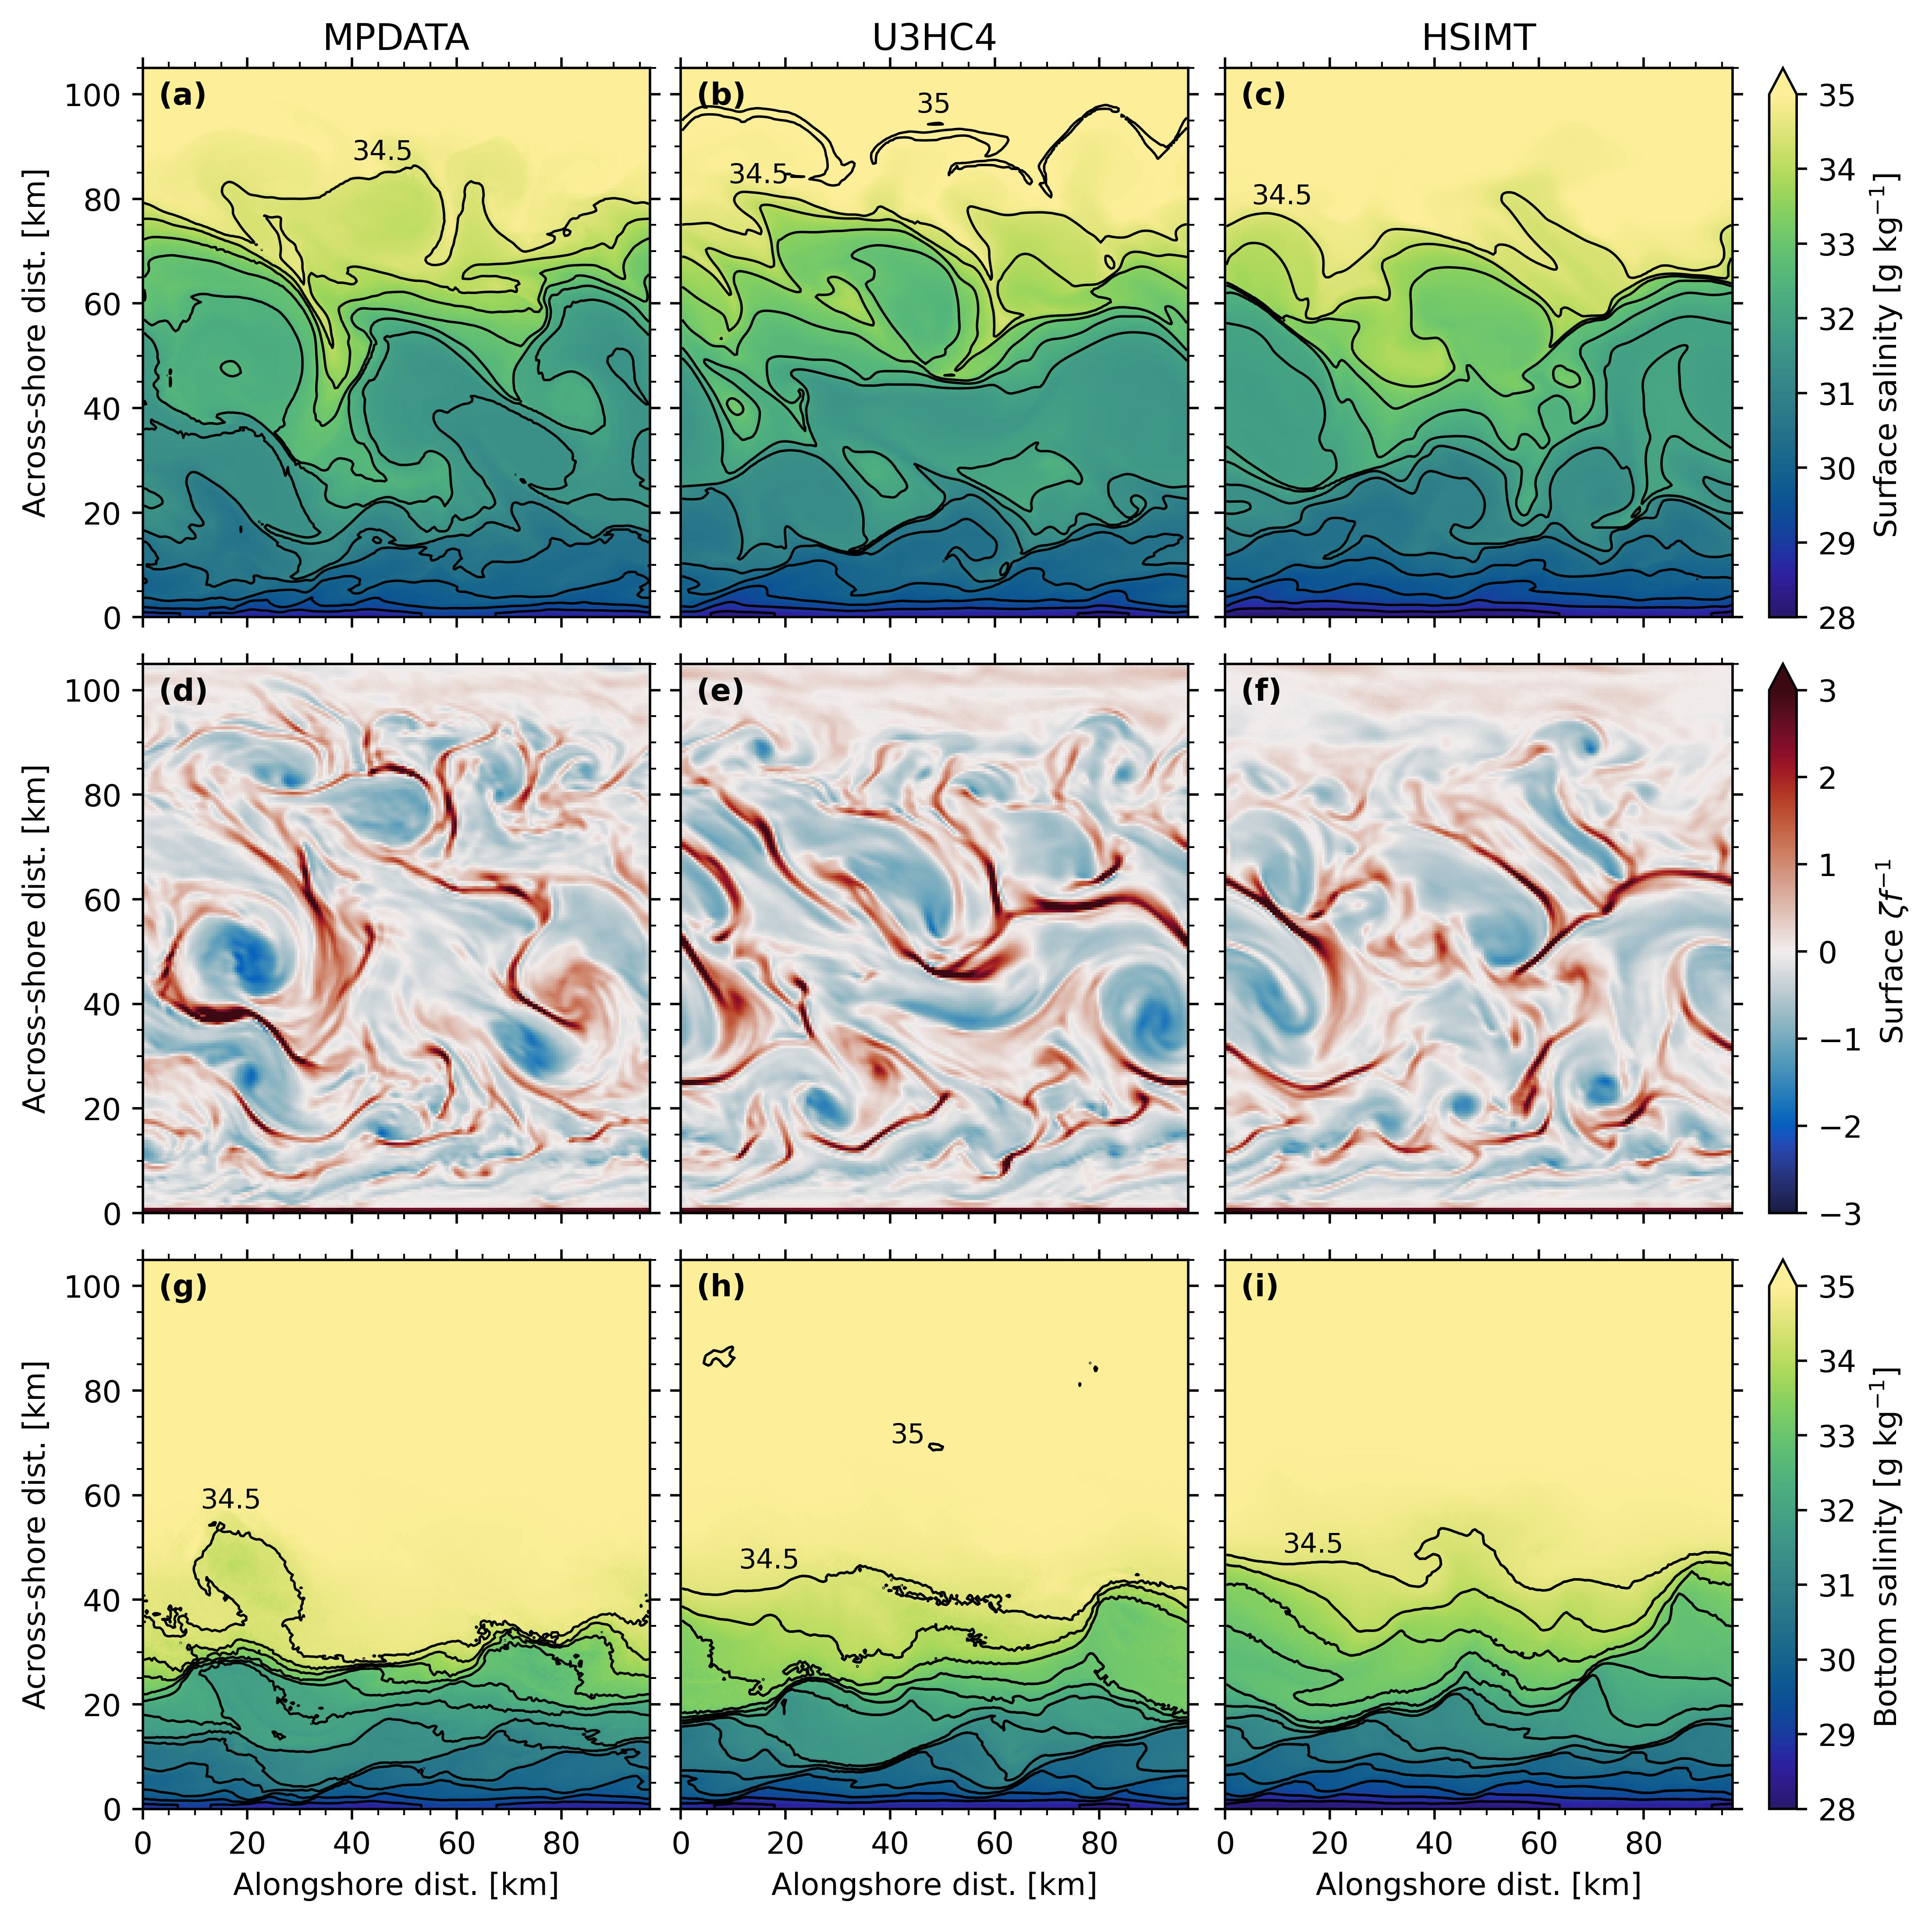
\includegraphics[width = 0.9\linewidth]{figures/shelfstrat_2024/shelf_dx_500_tadv_dt_30_day_30.jpg}\\
    \caption{Snapshots of surface salinity (a-c), surface $\zeta f^{-1}$ (d-f), and bottom salinity (g-i) on Day 30. Each column represents a different tracer advection scheme ensemble member with the largest $EKE_n$ on Day 30. Isohalines are shown every 0.5 g kg$^{-1}$ over the range of the colorbar in (a-c) and (g-i). The 35 g kg$^{-1}$ contours in the U3HC4 ensemble member are spurious.} \label{fig:isohalines}
     \end{center} 
\end{figure}

The volume-integrated double-averaged $APE$ is normalized by its initial value $APE_0$:
\begin{equation}
    APE_{n, ens} = \langle \overline{\iiint APE \, dV} \rangle \left[\overline{\iiint APE_0 \,dV}\right]^{-1}.
\end{equation}
$APE_{n, ens}$ is shown in Fig. \ref{fig:tadv_vol_int} (b) for each scheme and is consistent with arguments posed above. By day five, HSIMT has more $APE_{n, ens}$ than the other schemes and this grows with respect to time. U3HC4 has more $APE_{n, ens}$ than MPDATA for the entire simulation, although these differences remain marginal until day 15. The $APE_{n, ens}$ for all schemes decreases below their initial values, plateaus, then eventually rise above their initial values. The $APE_{n, ens}$ decreases as the isopycnal slope is reduced in the initially stratified region. Later increases in $APE_{n, ens}$ are caused by wind-induced mixing offshore of the eddy field where the isopycnal slope is controlled by temperature. There, wind mixing increases the isopycnal slope, which compensates for the $APE_{n, ens}$ decrease in the initially stratified region. If volume-integration were performed inshore of the initially stratified region, $APE_{n, ens}$ would continuously decline below its initial values (not shown). 

While the $EKE_{n, ens}$ remains similar between U3HC4 and MPDATA, differences in their bottom salinity structure (Fig. \ref{fig:isohalines} g-i) qualitatively support the idea that higher numerical mixing in U3HC4 reduces the amount of energy that can be extracted from the horizontal density gradient. That is, MPDATA isohalines are more pinched coast to the coast than U3HC4. Differences in the surface salinity structure also validate this argument (Fig. \ref{fig:isohalines} a-c) , with MPDATA experiencing the furthest offshore development of the 34.5 g kg$^{-1}$ isohaline. U3HC4 features spurious 35 g kg$^{-1}$ isohalines throughout the water column because the scheme is non-monotonic.  The argument that MPDATA and U3HC4 produce more-developed eddies is further supported with surface $\zeta f^{-1}$ (Fig. \ref{fig:isohalines}). In the end, the differences between U3HC4 and MPDATA are marginal. U3HC4 locally produces the sharpest fronts, but PDFs of $\zeta f^{-1}$ (not shown) are nearly identical.

Bulk values and ratios of the decomposed, ensemble-averaged integrated mixing quantities are shown in Tab. \ref{tab:mixing_tadv}. For example, the double-averaged, integrated total mixing is written as:
\begin{equation}
    \mathcal{M}_{tot,ens} = \langle \overline{\iiint \mathcal{M}_{tot} \, dV } \rangle
\end{equation}
and likewise for the physical $\mathcal{M}_{phy, ens}$ and numerical mixing $\mathcal{M}_{num,ens}$. HSIMT runs have substantially more numerical mixing than the other schemes and moderately less physical mixing. $\mathcal{M}_{phy,ens}$ constitutes 86\% of $\mathcal{M}_{tot,ens}$ for MPDATA, 83\% for U3HC4, and 66\% for HSIMT. $\mathcal{M}_{tot,ens}$ is very similar between the different advection schemes. 

\begin{table}[t]
\caption{Sensitivity of ensemble-averaged mixing quantities to the tracer advection scheme. Ratios of bulk (denoted by $\Sigma$) volume-integrated physical, numerical, and total mixing inshore of 97 km from Days 7.5-30. Note these are \textit{not} smoothed with a 16 hour rolling mean. Bulk values have units of 10$^7$(g kg)$^2$ m$^3$s$^{-1}$.} \label{tab:mixing_tadv}
\begin{center}
\begin{tabular}{cccccc}
\hline
Scheme & $\Sigma \mathcal{M}_{phy,ens}$& $\Sigma \mathcal{M}_{num,ens}$& $\Sigma \mathcal{M}_{tot,ens}$& $\mathcal{M}_{phy,ens}/\mathcal{M}_{tot,ens}$ & $\mathcal{M}_{num,ens}/\mathcal{M}_{tot,ens}$\\
\hline
MPDATA& 9.90& 1.59& 11.49& 0.86& 0.14  \\ 
U3HC4& 9.39& 1.98& 11.37& 0.83& 0.17 \\
HSIMT& 7.66& 3.88& 11.54& 0.66& 0.34 \\
\hline
\end{tabular}
\end{center}
\end{table}

Instantaneously, $\mathcal{M}_{num,ens}$ is larger in HSIMT runs relative to other schemes at all times. These results suggest that as instabilities form, the increased $\mathcal{M}_{num,ens}$ suppresses instability growth by preventing the release of $APE$. Weaker eddies decrease the relative amount of $\mathcal{M}_{phy,ens}$ because they do not penetrate as deeply into the water column. Therefore, the impacts of $\mathcal{M}_{num,ens}$ on the larger-scale flow are similar to larger-scale models and \textit{not} like an implicit LES discussed in Section 1. In other words, the solution is sensitive to the type of mixing that occurs, even if the $\mathcal{M}_{tot,ens}$ is similar between different advection schemes.

Finally, we provide quantitative estimates of the differences in salinity structure between the advection schemes. This is done using cross-sections of alongshore- and ensemble-averaged salinity ($\overline{\overline{s}}$) on days 7.5 and 30 for MPDATA and the relative differences $\Delta \overline{\overline{s}}$ with other schemes are shown in Fig. \ref{fig:cs_salt}. This allows us to examine whether the differences in salinity structure shown in Fig. \ref{fig:isohalines} are robust and not due to analysis of the highest $EKE$ ensemble members. Alongshore- and ensemble-averaged isopycnals are also overlaid every 0.5 kg m$^{-3}$. The 1027 kg m$^{-3}$ isopycnal approximately represents the boundaries of the salinity stratified region (Fig. \ref{fig:cs_salt} a).

\begin{figure}[t!]
    \begin{center}
    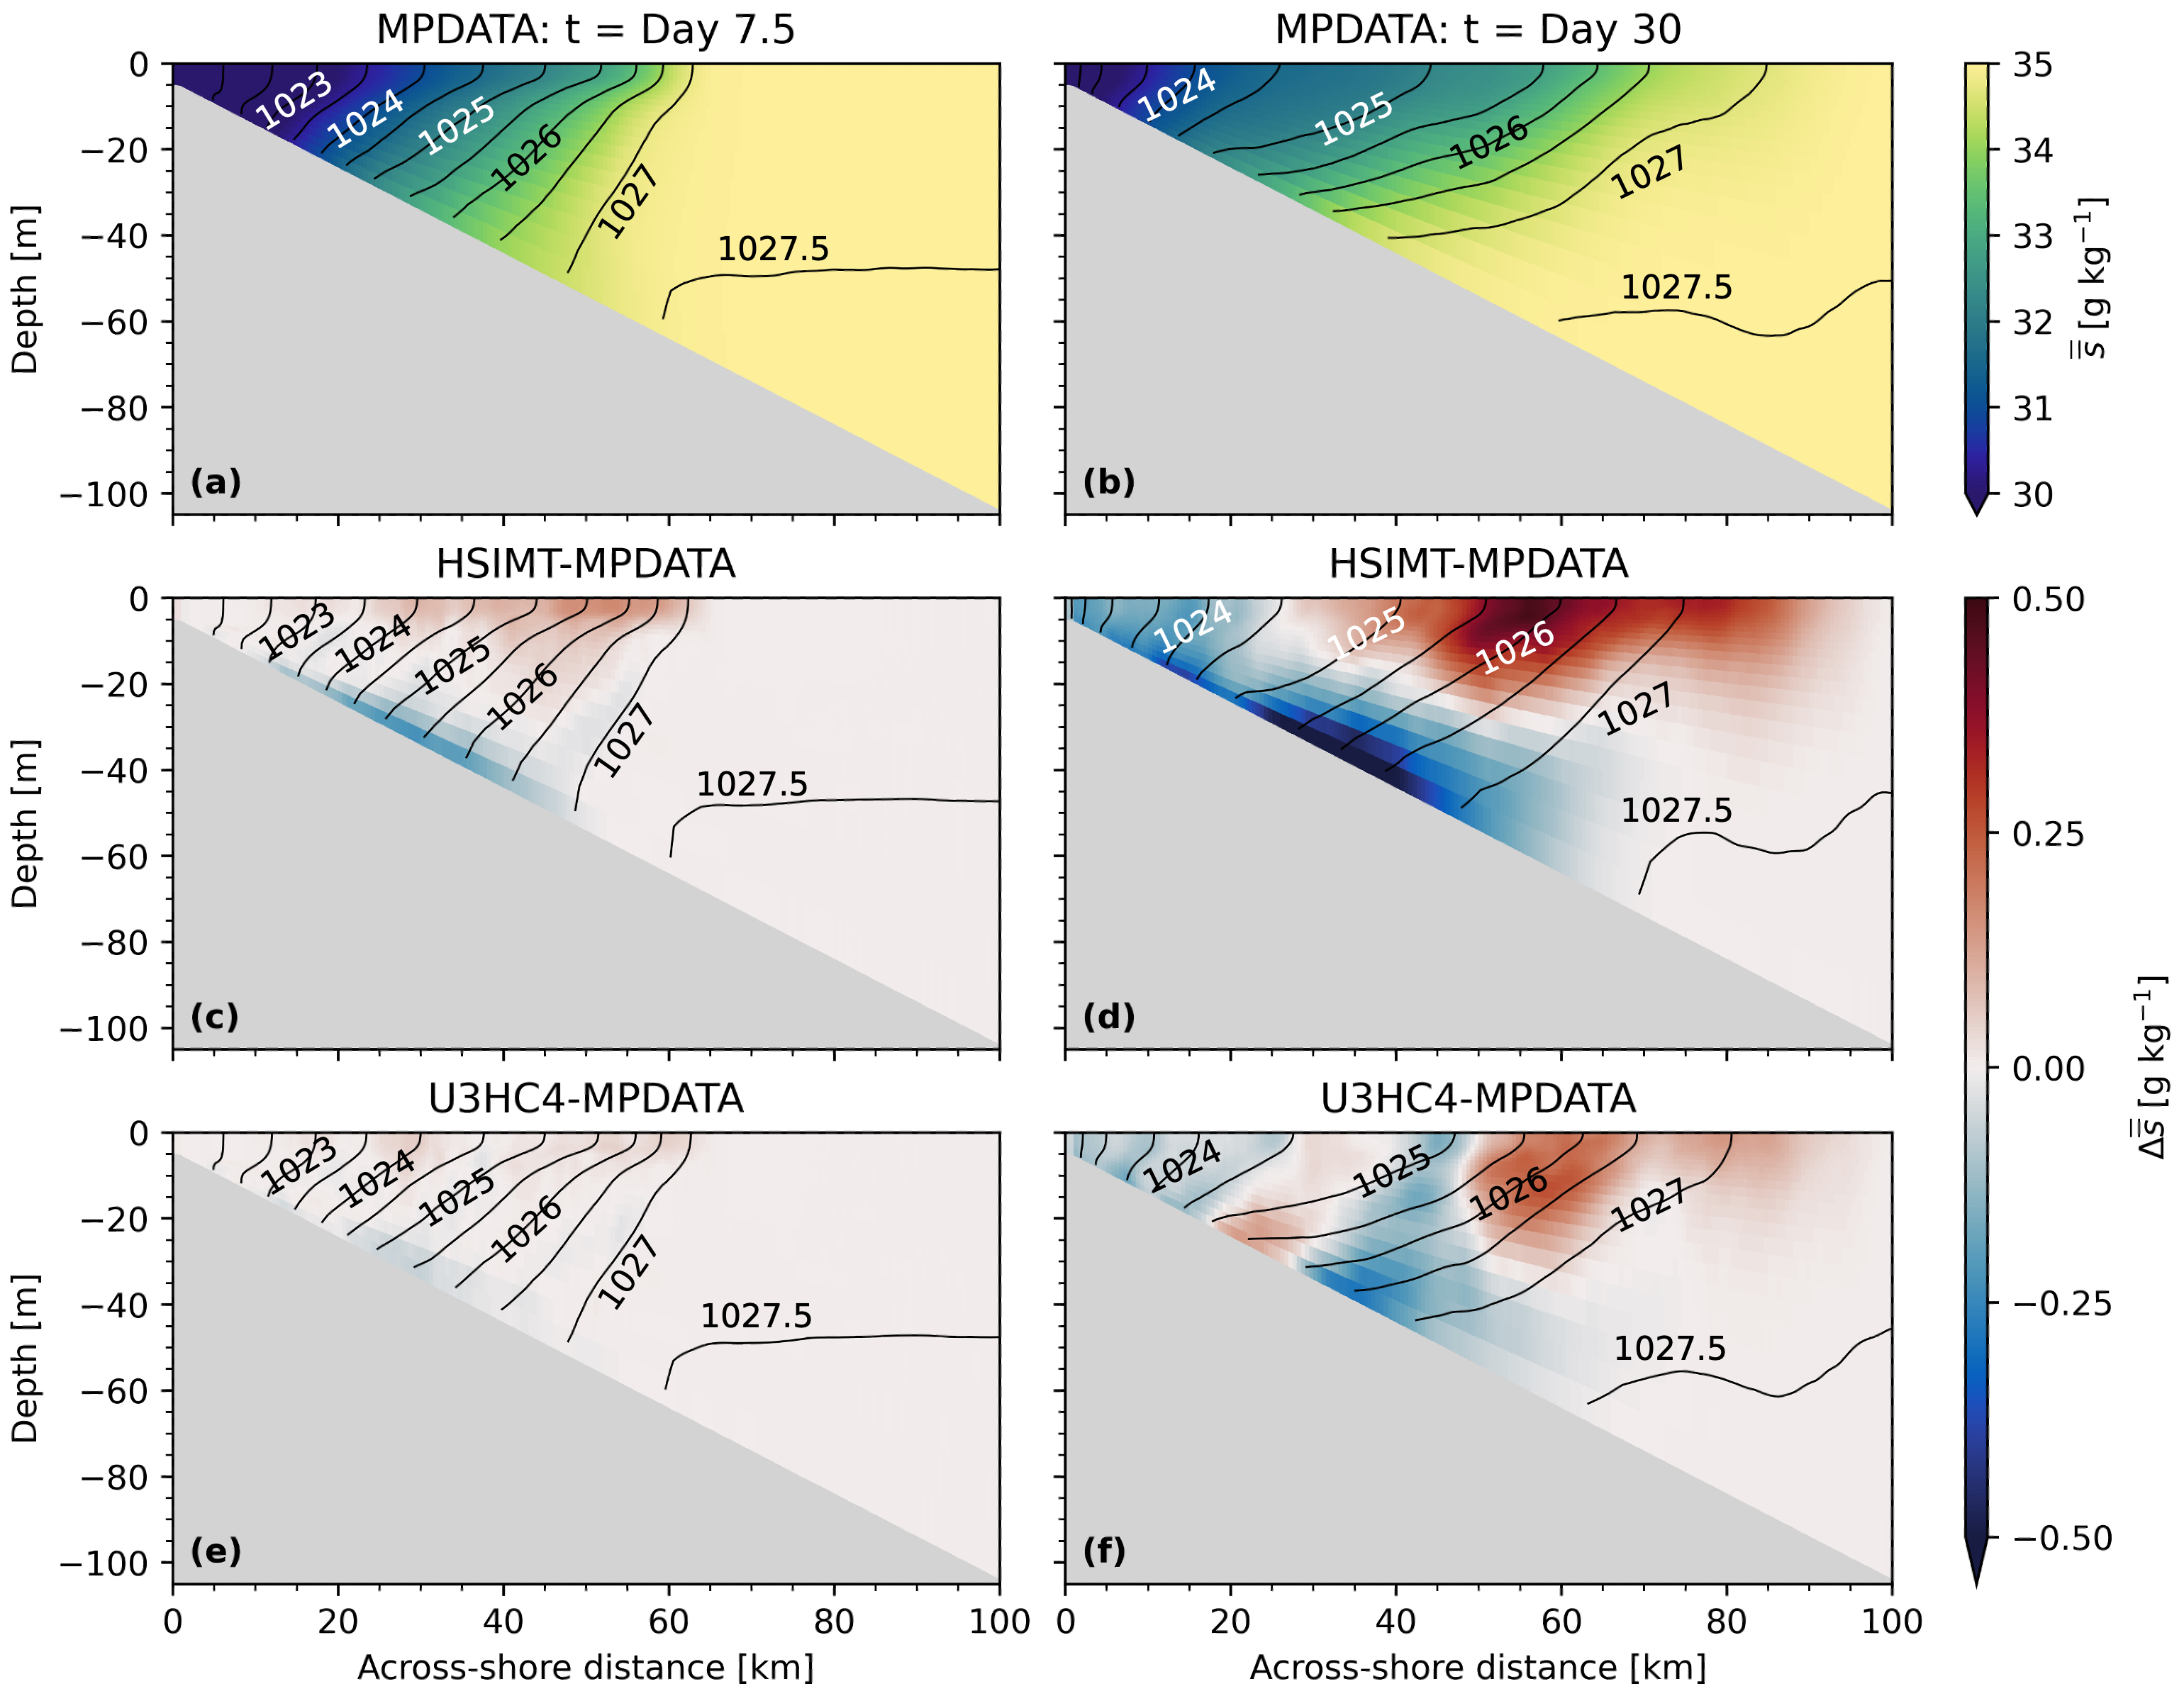
\includegraphics[width = \linewidth]{figures/shelfstrat_2024/tadv_cs_salt_isopyc.jpg}\\
    \caption{Cross-sections of alongshore- and ensemble- averaged salinity (indicated by double overline) for MPDATA on Days 7.5 (a) and 30 (b). Relative differences between the same quantities for HSIMT (c-d) and U3HC4 (e-f). Isopycnals are overlaid every 0.5 kg m$^{-3}$ for each scheme. Note the bathymetry noise is smoothed by the averaging, so the isopycnals do not appear to reach the seafloor.} \label{fig:cs_salt}
     \end{center} 
\end{figure}

On day 7.5, $\Delta \overline{\overline{s}}$ between HSIMT and MPDATA is small, with a two layer structure that is fresher near the bottom and saltier from the middle of the water column to the surface (Fig. \ref{fig:cs_salt} c).  The differences between U3HC4 and MPDATA are lesser, and $\Delta \overline{\overline{s}}$ is slightly fresher towards the bottom inshore of the initially stratified region and saltier near the surface (Fig. \ref{fig:cs_salt} e). Differences in isopycnal structure between schemes are marginal on day 7.5, but by day 30, the mean isopycnal slope has reduced for all advection schemes. The surface position of the 1027 kg m$^{-3}$ isopycnal is approximately 10 km further offshore in the MPDATA case than in the HSIMT case and five km further offshore in the  MPDATA case than in the U3HC4, consistent with previous arguments. 

On day 30, $\Delta\overline{\overline{s}}$ between HSIMT and MPDATA is saltier by up 0.5 g kg$^{-1}$ in the upper half of the water column offshore of 30 km. In the lower half of the water column, $\Delta\overline{\overline{s}}$ is fresher by over -0.75 g kg$^{-1}$ close to the bottom. Inshore of 30 km, $\Delta \overline{\overline{s}}$ is persistently fresher. Regarding U3HC4, $\Delta \overline{\overline{s}}$ is smaller in magnitude than HSIMT nearly everywhere except for a saltier band that extends diagonally through the water column from 15-40 km.

\section{Discussion} \label{sec:discussion}

Previous studies suggest numerical mixing impacts the larger-scale flow and tracer structure differently than physical mixing in simulations of estuarine and coastal flows using primitive equation models \citep{fofonova2021plume, Kalra_2019, karna2016evaluation, Ralston_2017}. However, these studies come with one of the following caveats or challenges: 1) mixing is not quantified directly or online \citep{fofonova2021plume, karna2016evaluation}, 2) the domains are highly idealized \citep{fofonova2021plume, Kalra_2019}, and 3) quantitative relationships between numerical mixing and model skill in realistic domains requires an extensive array of field observations \citep{karna2016evaluation, Ralston_2017}. The current study is novel because we explicitly quantify the numerical mixing in an idealized domain that is able to realize a complex ocean state that resembles conditions in a realistic simulation. While the base case is not fully realistic due to the idealized bathymetry and lack of river forcing, eddy structure (Fig. \ref{fig:base_case_plan}) and frontogenesis/frontolysis (Fig. \ref{fig:jpdf}) are representative of the realistic model. The idealized domain allows for a large ensemble of simulations, as well as clear metrics for comparisons across the ensemble through alongshore averages.

A primary result of our study is that excessive numerical mixing can damp the release of $APE$ by suppressing submesoscale baroclinic instabilities. To demonstrate this, we varied numerical mixing through the choice of advection scheme, each with different numerical mixing, in order to relate an alongshore average state to the magnitude of numerical mixing. Even though simulations using all of the different advection schemes are submesoscale eddy-resolving, in that they all have qualitatively similar energetic eddy fields, $\mathcal{M}_{num}$ impacts the larger-scale flow and tracer fields in such a way that simulations with higher numerical mixing have higher integrated $APE$ and lower integrated $EKE$, indicating the suppression of baroclinic instabilities that release $APE$. Thus, numerical mixing is quite distinct from, e.g., models that use numerical mixing only to remove energy at the grid scale in a downward cascade toward small scales, discussed in Section 1. In other words, though the numerical mixing is primarily at the fronts, the submesoscale eddies themselves are altered such that their impact on altering the initial state is reduced.

$\mathcal{M}_{num}$ dominates $\mathcal{M}_{phy}$ in frontal zones due to their sharp lateral salinity gradients, consistent with previous studies \citep{Kalra_2019, Holmes_2021, Ralston_2017, Wang_2021}. Our analysis of $nFGF$ in the surface layer of both models suggest the strongest $\mathcal{M}_{num}$ occurs in intense regions of frontogenesis and frontolysis. However, frontogenesis produces stronger $\mathcal{M}_{num}$ than frontolysis because the horizontal gradients are actively being sharpened. $\mathcal{M}_{num}$ is significant within the mixed layer and dominates at shallow depths (e.g., the top one m of the water column) where $\mathcal{M}_{phy}$ is weak because of weak vertical tracer gradients. These results suggest mixing processes within frontal zones may be predominantly driven by $\mathcal{M}_{num}$. Future studies may use our results as a blueprint to investigate the impacts of $\mathcal{M}_{num}$ on specific processes such as symmetric instability \citep{dong2021scale} or the subduction of surface waters due to inertially-modulated frontal convergence \citep{qu2022rapid}.

A limitation of this study is that we had to vary the tracer advection scheme to understand the impacts of $\mathcal{M}_{num}$. An implicit assumption is that MPDATA simulations are taken to be the ``truth'' because they produce the most developed instabilities, however, this should be treated with caution because analytical solutions are unavailable. \citet{Kalra_2019} examined the same advection schemes in a suite of idealized experiments and did not not observe excessive $\mathcal{M}_{num}$ with HSIMT. Since our model is idealized, it is unclear if the trends observed in this study will translate to realistic numerical simulations. In addition, although U3HC4 produced a similar eddy field to MPDATA, spurious water formation may be problematic for estuarine and coastal flows where significant lateral freshwater forcing is present. 

Another limitation of this study is that we did not add explicit horizontal mixing, which has been shown to reduce $\mathcal{M}_{num}$ \citep{Griffies_2000,Holmes_2021,Ilicak_2012}. It is worth noting that HSIMT run times were 40\% faster on average than MPDATA and 32\% faster than U3HC4, although the simulations were not optimized for computational efficiency. The relative differences in computational efficiency between these schemes has been suggested previously \citep{wu2010advection, wu2023evaluation} but requires more investigation. Thus, future studies may tune the lateral mixing scheme to leverage HSIMT's increased computational efficiency in realistic simulations if unacceptable levels of numerical mixing are found. 

\section{Conclusions} \label{sec:conclusions}

The primary finding of this study is that excessive numerical salinity mixing partially suppresses submesoscale baroclinic instabilities. We showed this with an idealized ROMS model of the TXLA shelf developed by \citet{Hetland_2017} in a modified domain with oscillatory near-inertial wind forcing. Use of the idealized model was motivated by results from an $\mathcal{O}(300 \, \text{m})$ realistic simulation \citep{Schlichting23}. In both models, numerical mixing dominates physical mixing in frontal zones and remains significant within the mixed layer, consistent with previous studies. Our focus was understanding the impacts of numerical mixing on the larger-scale ocean state and tracer fields. Future work with front refined simulations may use these results as a template to investigate how specific frontal processes such as symmetric instability or inertially-modulated frontogenesis are affected by numerical mixing.  

First, we identified and analyzed a base case relative to a case with no wind forcing. The base case was selected from an ensemble with variable oscillatory, near-inertial wind stress amplitude. Joint probability density functions of the normalized frontogenesis function and numerical mixing indicate the sharpening and destruction of horizontal salinity gradients in the base case well represents the realistic model. The base case also had the maximum ratio of numerical to physical mixing relative to the other ensemble members, which made the impacts of numerical mixing easier to identify. 

Then, we tested the sensitivity of the base case with three tracer advection schemes (MPDATA, U3HC4, and HSIMT) to examine how changing mixing rates affect instability growth. We performed ensemble runs with variable bathymetry to ensure differences between schemes were robust. Instability development was evaluated with several analysis methods: volume-integrated $EKE$, $APE$, surface and bottom isohaline position, and alongshore averaged salinity and density sections. While the bulk total mixing remained similar between each schene, HSIMT runs featured over double the numerical mixing and $\sim$20\% less physical mixing. HSIMT runs featured weaker $EKE$, higher $APE$, reduced offshore spreading/variability of surface isohalines relative to the initially stratified region, and increased isopycnal slope. Numerical mixing prevented the release of $APE$, which suppressed the growth of instabilities. MPDATA featured a slightly more developed eddy field relative to U3HC4 but required the longest run times. U3HC4 runs featured spurious water formation as a result of the schemes non-monotonicity. While insignificant for the U3HC4 runs, the inaccuracies caused by spurious numerical mixing are likely to be more problematic in simulations that include freshwater fluxes, where negative salinity water could be created. These schemes should be tested in future studies with realistic simulations so their benefits and drawbacks may be better understood. 

\section*{Data availability statement}
Model analysis was done in Python ver 3.9 and the accompanying code is available at \url{https://zenodo.org/records/10735283}. Output for the realistic TXLA model are available at \url{https://hafen.geos.tamu.edu/thredds/catalog/catalog.html}. Output from the idealized simulations is available upon request.

\section*{Acknowledgements}
This material is based upon work done in the Study for Exascale Advances in a High-resolution Ocean using ROMS Coupled to E3SM (SEAHORCE) project, supported by the U.S. Department of Energy (DOE), Office of Science, Office of Advanced Scientific Computing Research, and Office of Biological and Environmental Research, Scientific Discovery through Advanced Computing (SciDAC) program. D.S. was funded by NSF grant OCE-1851470. R.H. were funded by the ICoM project, a U.S. DOE grant. Texas A\&M high performance research computing resources were used to produce all numerical simulations. D.S. thanks Ping Chang for helpful discussions while preparing this manuscript. We thank the anonymous reviewers whose comments improved this manuscript. 

